% MATEMÁTICAS PARA LA CIENCIA DE DATOS

\documentclass[
%xcolor={dvipsnames},
%hyperref={colorlinks}
%twoside,
%12pt,
%letterpaper
%]{amsbook}
%]{tufte-book}
]{WileySix}
%,graybox,envcountchap,sectrefs]{svmono}
\usepackage{fontenc}
\usepackage{graphicx}
\usepackage[utf8]{inputenc}
\usepackage[spanish,mexico]{babel}
\usepackage{fontenc}
\usepackage{amsmath}
\usepackage{amssymb}
\usepackage{graphicx}
\usepackage{mathrsfs}
\usepackage{yfonts}
\usepackage{enumerate}
\usepackage{mathtools}
\usepackage{textcomp}
\usepackage{lmodern}
\usepackage{fancyvrb}
\usepackage{multicol}
\usepackage{wrapfig}
\usepackage{floatflt}
\usepackage{filecontents}
\usepackage{hyperref}
\usepackage{bibentry}
\usepackage{graphicx} % Allows including images
\usepackage{booktabs} % Allows the use of \toprule,
%\usepackage{mdframed}
\usepackage[dvipsnames]{xcolor}
\usepackage{tikz}
\usetikzlibrary{matrix,arrows,decorations.pathmorphing}

\usepackage{amsthm}

 \usepackage{hyperref}
\hypersetup{
	colorlinks=true,
	linkcolor=Green,
	filecolor=Green,
	citecolor = Green,      
	urlcolor=Green,
}

%%% MANDATORY!!!

\newcommand{\R}{\mathbb{R}}
\newcommand{\N}{\mathbb{N}}
\newcommand{\Q}{\mathbb{Q}}
\newcommand{\C}{\mathbb{C}}
\newcommand{\Z}{\mathbb{Z}}

\newcommand{\set}[1]{\left\{ #1 \right\}}
\newcommand{\evat}[2]{\left. #1 \right|_{#2}}
\newcommand{\sett}[2]{\left\{ \left.#1 \right| #2 \right\} }

\newcommand{\inp}[1]{\langle #1 \rangle}
\newcommand{\norm}[1]{\left\| #1 \right\|}
\newcommand{\abs}[1]{\left|#1\right|}
\newcommand{\imply}{\rightarrow}

%precalculo

\newcommand{\mcd}{mcd}
\newcommand{\mcm}{mcm}

% Calculo
\newcommand{\del}{\delta}
\renewcommand{\a}{\alpha}
\newcommand{\Del}{\Delta}
\newcommand{\sech}{sech}
\newcommand{\csch}{csch}
\newcommand{\ep}{\epsilon}
\newcommand{\p}{\partial}

%ecuaciones diferenciales
\newcommand{\lap}[1]{\mathcal{L}\set{#1}}
\newcommand{\lapin}[1]{\mathcal{L}^{-1}\set{#1}}
\newcommand{\lam}{\lambda}

%álgebra lineal

\renewcommand{\a}{\alpha}
\renewcommand{\b}{\beta}

\newcommand{\gen}[1]{\operatorname{gen}\left( #1 \right)}

\newcommand{\av}{\arrowvert}

\newcommand{\id}{\operatorname{Id}}

\newcommand{\im}{\mathfrak{I}}

\renewcommand{\Im}{\operatorname{Im}}

\newcommand{\nul}[1]{\operatorname{nul}\left( #1 \right)}
\newcommand{\ran}[1]{\operatorname{ran}\left( #1 \right)}

\newcommand{\ssi}{\Leftrightarrow}
\newcommand{\basis}[1]{\left( #1 \right)}
\renewcommand{\th}{\theta}
\renewcommand{\arg}[1]{\varphi(#1)}
\newcommand{\bm}[1]{\begin{bmatrix}#1\end{bmatrix}}

%\renewtheorem{frame}{}

\newtheorem{thm}{Teorema}[section]
\newtheorem{prop}{Propiedad}[section]
\newtheorem{lem}{Lema}[section]
\newtheorem{cor}{Corolario}[section]
\newtheorem{alg}{Algoritmo}[section]
\newtheorem{ans}{Respuesta}[section]


\theoremstyle{definition}
\newtheorem{defn}{Definición}[section]
\newtheorem{exmp}{Ejemplo}[section]
\newtheorem{axiom}{Axioma}[section]
%\newtheorem{exmp}{Ejemplo}[section]


\theoremstyle{remark}
\newtheorem{rem}{Observación}[section]
\newtheorem{ilu}{Ilustración}[section]
\newtheorem*{hint}{Sugerencia}

\newenvironment{sol}{\begin{proof}[Solución]}{\end{proof}}
\newcommand{\f}{\phi}
\newcommand{\vphi}{\varphi}
\newcommand{\vf}{\varphi}
\newcommand{\flow}[2]{\varphi^{#1}\left( #2 \right)}
\renewcommand{\d}[1]{\dot{#1}}
\renewcommand{\r}{\rho}
\newcommand{\A}{\mathcal{A}}
\newcommand{\gam}{\gamma}
\renewcommand{\a}{\alpha}
\renewcommand{\b}{\beta}
\newcommand{\om}{\omega}
\newcommand{\iso}{\simeq}
\newcommand{\tensor}{\otimes}
\newcommand{\inc}{\hookrightarrow}
\renewcommand{\L}{\mathcal{L}}
\renewcommand{\H}{\mathcal{H}}
\newcommand{\D}{\mathcal{D}}
\newcommand{\converge}[1]{\xrightarrow{#1}}
\newcommand{\cott}[1]{T^{*}\T^{#1}}
%\newcommand{\G}{\mathcal{G}}
\newcommand{\hu}{\textbf{h}}
\newcommand{\deck}[1]{\operatorname{Dake}\left( #1 \right)}
\newcommand{\til}[1]{\tilde{#1}}
\newcommand{\Gam}{\Gamma}
\newcommand{\grad}{\nabla}
\newcommand{\var}{\Delta}
\newcommand{\avch}[2]{\frac{\Delta #1}{\Delta #2}}
\newcommand{\Avch}[2]{\dfrac{\Delta #1}{\Delta #2}}
\newcommand{\Err}{\operatorname{Err}}
\newcommand{\wed}{\wedge}
\newcommand{\biconditional}{\longleftrightarrow}
\newcommand{\yields}{\vdash}
\newcommand{\onlyif}{\Rightarrow}
\newcommand{\uset}{\mathbb{U}}
\newcommand{\minus}{\backslash}
\newcommand{\symdif}{\oplus}
\newcommand{\rel}[1]{\boxed{{\color{blue}\textbf{#1}}}}
\newcommand{\dom}[1]{\operatorname{Dom}\left( #1 \right)}
\newcommand{\nrel}[1]{\boxed{{\color{red}\not}{\color{orange}\textbf{#1}}}}
\newcommand{\comp}[2]{#1 \circ #2}

\theoremstyle{definition}
  \newtheorem{conj}{Conjectura}%[section]
%  \newtheorem{prob}{Problema}%[section]
  \newtheorem*{ax}{Axioma}
  \newtheorem{tdv}{Tabla de Verdad}

\theoremstyle{remark}
  \newtheorem{claim}{Afirmación}%[section]
  %\newtheorem{rem}{Observación}[chapter]
  %\newtheorem*{note}{Nota}
  \newtheorem{case}{Caso}


\renewcommand{\d}[1]{\dot{#1}}
\renewcommand{\r}{\rho}
\renewcommand{\a}{\alpha}
\renewcommand{\b}{\beta}
\renewcommand{\L}{\mathcal{L}}
\renewcommand{\H}{\mathcal{H}}

\newcommand{\Var}{\operatorname{Var}}
\newcommand{\s}{\sigma}
\newcommand{\comb}[2]{\begin{pmatrix} #1 \\ #2\end{pmatrix}}
\newcommand{\cov}{\operatorname{Cov}}


\title{Optimización y combinatoria}
\author[J. Castillo]{Juliho Castillo Colmenares}

\begin{document}
	\maketitle
	\tableofcontents

\chapter{Matemáticas Discretas}
\section{L\'ogica y C\'alculo Proposicional}


    Muchos algoritmos y demostraciones usan expresiones l\'ogicas tales como
    \texttt{si p entonces q}. Entonces es necesario conocer los casos en los cuales esas expresiones son \texttt{ciertas} o \texttt{falsas}. Discutiremos esto en esta unidad. 





    Tambi\'en investigamos el valor de verdad de enunciados cuantificados, que son aquellos que usan los cuantificadores l\'ogicos \texttt{para todo...} y \texttt{existe...}


\subsection{Proposiciones y Declaraciones Compuestas}


    Una proposici\'on es un enunciado declarativo que puede ser cierto o falso, pero no ambos. 



    \begin{exmp}
        ?`Cu\'al de los siguientes enunciados es una proposici\'on?
        \begin{multicols}{2}
            \begin{enumerate}
                \item El hielo flota en el agua.
                \item China est\'a en Europa.
                \item $2+2=4$
                \item $2+2=5$
                \item ?`A donde vas?
                \item Haz tu tarea.
            \end{enumerate}
        \end{multicols}
    \end{exmp}
    


\subsection{Proposiciones compuestas}


    Muchas proposiciones est\'an \texttt{compuestas} de proposiciones m\'as simples, llamadas \emph{subproposiciones}, por medio de \emph{conectores l\'ogicos.}  Una proposici\'on se dice que es \emph{primitiva} si no puede descomponerse en proposiciones m\'as simples.



    Por ejemplo, las siguientes proposiciones son compuestas
    \begin{itemize}
        \item ``Las rosas son rojas y las violetas son azules''
        \item ``Juan es inteligente y estud\'ia hasta muy noche''
    \end{itemize}
    



    La propiedad fundamental de una proposici\'on compuesta es que su valor de verdad est\'a completamente deteminado por los valores de verdad de sus subproposiciones y la manera en la cual est\'an conectadas para formar la proposici\'on compuesta. 


\subsection{Operaciones L\'ogicas B\'asicas}


    En esta secci\'on discutiremos las tres operaciones l\'ogical b\'asicas: conjunci\'on , disjunci\'on  y la negaci\'on.


\subsection{Conjunci\'on $p \wed q$}


    Cualesquiera dos proposiciones $p,q$ pueden ser combinadas por la palabra ``y'' para formar una proposici\'on compuesta llamada \emph{conjunci\'on} que se escribe $p\wed q.$



    \begin{defn}
        Si tanto $p$ como $q$ son ciertas, entonces $p \wed q$ es cierta; en otro caso $p\wed q$ es falsa.
    \end{defn}
    



    \begin{rem}
        Para entender mejor como se conectan los valores de verdad, generalmente se utilizan \emph{tablas de verdad.}  
        
        Por brevedad $1$ representar\'a el valor \texttt{cierto}, mientras que $0$ representar\'a \texttt{falso}
    \end{rem}
    



    \begin{tdv}[Conjunci\'on]
        \label{tdv:and}
        \begin{center}
            \begin{tabular}{|l|l|l|}\hline
                $p$ & $q$ & $p \wed q$\\\hline
                1 & 1 & 1\\\hline
                1 & 0 & 0\\\hline
                0 & 1 & 0\\\hline
                0 & 0 & 0\\\hline
            \end{tabular}
        \end{center}
        
    \end{tdv}
    



    En este curso, usaremos el \emph{sistema algebr\'aico de computo} \texttt{SageMath}, el cu\'al est\'a escrito con base en el lenguaje de programaci\'on \texttt{Python} e incorpora diversos paquetes de \texttt{OpenSource}.
    
    
    Puede acceder a este sistema, a trav\'es de \href{https://cloud.sagemath.com/}{https://cloud.sagemath.com/} 
    



    Construimos la tabla de verdad de la conjunci\'on en el siguiente scritp \href{https://cloud.sagemath.com/projects/12787063-cafe-4f3b-a2e0-905f8b83cf3b/files/MD01_TRDV01_AND.sagews}{https://goo.gl/hEF5os}
    \begin{center}
        
\includegraphics[height=5cm,keepaspectratio=true]{./md/MD01_TDV01_AND.png}
        % MD01_TDV01_AND.png: 0x0 pixel, 300dpi, 0.00x0.00 cm, bb=
    \end{center}
    



    \begin{exmp}
        ?`Cu\'al de las siguientes proposiciones es cierta?
        
        \begin{enumerate}
            \item El hielo flota y $2+2=4$
            \item El hielo flota y $2+2=5$
            \item China est\'a en Europa y $2+2=4$
            \item China est\'a en Europa y $2+2=5$
        \end{enumerate}
        
    \end{exmp}
    


\subsection{Disjunci\'on $p \vee q$}


    Cualesquiera dos proposiciones $p,q$ pueden ser combinadas por la palabra ``o'' para formar una proposici\'on compuesta llamada \emph{disjunci\'on} que se escribe $p \vee q .$



    \begin{defn}
        Si tanto $p$ como $q$ son falsas, entonces $p \vee q$ es falsa; en otro caso $p\vee q$ es verdadera.
    \end{defn}
    




    \begin{tdv}[Disjunci\'on]
        \label{tdv:or}
        \begin{center}
            \begin{tabular}{|l|l|l|}\hline
                $p$ & $q$ & $p \vee q$\\\hline
                1 & 1 & 1\\\hline
                1 & 0 & 1\\\hline
                0 & 1 & 1\\\hline
                0 & 0 & 0\\\hline
            \end{tabular}
        \end{center}
        
    \end{tdv}
    



    Construimos la tabla de verdad de la disjunci\'on en el siguiente scritp \href{https://cloud.sagemath.com/projects/12787063-cafe-4f3b-a2e0-905f8b83cf3b/files/MD01_TDV02_OR.sagews}{https://goo.gl/5kXzNI}
    \begin{center}
        
\includegraphics[height=5cm,keepaspectratio=true]{./md/MD01_TDV02_OR.png}
        % MD01_TDV01_AND.png: 0x0 pixel, 300dpi, 0.00x0.00 cm, bb=
    \end{center}
    



 \begin{rem}
  Algunas veces \texttt{``p o q''} se entiende en el sentido exclusivo: Puede ocurrir \texttt{p} o \texttt{q}, \emph{pero no ambos,} que es diferente a la definici\'on anterior. Sin embargo, existe un conector llamado de hecho \texttt{o exclusivo,} que cumple esta definici\'on y consideraremos m\'as adelante. 
 \end{rem}



\subsection{Negaci\'on $\neg p$}


 Dada cualquier proposici\'on $p,$ otra proposici\'on llamada \emph{negaci\'on} de $p$ puede ser formada escribien \emph{``No es cierto que...''} o \emph{``Es falso que...''} antes de \texttt{p}.
 
 De manera m\'as sencilla, decimos \texttt{no $p$} y escribimos $\neg p.$



 
\begin{defn}[Negaci\'on]
 Si $p$ es cierta, entonces $\neg p$ es falsa; pero si $p$ es falsa, $\neg p$ es cierta.
\end{defn}




    \begin{tdv}[Negaci\'on]
        \label{tdv:not}
        \begin{center}
            \begin{tabular}{|l|l|}\hline
                $p$ & $\neg p$\\\hline
                1 & 0 \\\hline
                0 & 1 \\\hline
            \end{tabular}
        \end{center}
        
    \end{tdv}
    



    Construimos la tabla de verdad de la disjunci\'on en el siguiente scritp \href{https://cloud.sagemath.com/projects/12787063-cafe-4f3b-a2e0-905f8b83cf3b/files/MD01_TDV03_NOT.sagews}{https://goo.gl/sgCfkC}
    \begin{center}
        
\includegraphics[height=5cm,keepaspectratio=true]{./md/MD01_TDV03_NOT.png}
        % MD01_TDV01_AND.png: 0x0 pixel, 300dpi, 0.00x0.00 cm, bb=
    \end{center}
    


\subsection{Proposiciones y Tablas de Verdad}


 Sea $P(p,q,...)$ una expresi\'on construida con variables l\'ogicas $p,q,...,$ que toman valores de \texttt{verdadero ``V''} o \texttt{falso ``F''}, a trav\'es de conectores l\'ogicos como $\wed, \, \vee, \, \neg$ y otros  que discutiremos m\'as adelante.
 
 
 Tales expresiones $P(p,q,...)$ son llamadas \emph{proposiciones.}



 La propiedad principal de una proposici\'on $P(p,q,...)$ es que sus valores de verdad s\'olo dependen del valor de sus varibles. 
 
 
 Una manera simple y concisa de mostrar esta relaci\'on es a trav\'es de una \emph{tabla de verdad.}



 \begin{exmp}
  Contruir la tabla de verdad de la proposici\'on
  $$\neg \left( p \wed \neg q \right).$$
 \end{exmp}




 Construimos la tabla de verdad de la proposici\'on anterior con el siguiente script \href{https://goo.gl/V2Axzi}{https://goo.gl/V2Axzi}
\begin{center}
        
\includegraphics[height=5cm,keepaspectratio=true]{./md/MD01_TDV04.png}
        % MD01_TDV01_AND.png: 0x0 pixel, 300dpi, 0.00x0.00 cm, bb=
\end{center}
 



 \begin{tdv}[$\neg\left( p \wed \neg q \right)$] 
  \begin{tabular}{lllll}
p & q & not q & p and not q & not( p and not q) \\
$1$ & $1$ & $0$ & $0$ & $1$ \\
$1$ & $0$ & $1$ & $1$ & $0$ \\
$0$ & $1$ & $0$ & $0$ & $1$ \\
$0$ & $0$ & $1$ & $0$ & $1$ \\
\end{tabular}
 \end{tdv}




 \begin{rem}
  Para evitar el uso excesivo de parentesis, algunas veces adoptamos una jerarqu\'ia para los conectores l\'ogicos. 
  
  
  De manera especifica $\neg$ tiene prioridad sobre $\wed,$ que a su vez tiene prioridad sobre $\vee$.
 \end{rem}



 Por ejemplo, $$\neg p \wed q$$ significa $$\left( \neg p \right) \wed q$$  y no
 $$
 \neg(p \wed q).
 $$



 \subsection{M\'etodo alternativo de construir una tabla de verdad}
\begin{center}
\begin{tabular}{|l|l|l|l|l|l|l|}\hline
 $p$ & $q$ & $\neg$ & $(p$ & $\wed$ & $\neg$ & q) \\\hline
 $1$ & $1$ &  &  & &  & \\\hline
 $1$ & $0$ &  &  & &  & \\\hline
 $0$ & $1$ &  &  & &  & \\\hline
 $0$ & $0$ &  &  & &  & \\\hline
\end{tabular}
\end{center}




\begin{exmp} Construya las tablas de verdad de las siguientes proposiciones
\begin{enumerate}
 \item $p\vee \neg p$
 \item $p\wed \neg p$
 \item $\neg\left( p \vee q \right)$
 \item $\neg p \wed \neg q$
 \item $\neg\left( p \wed q \right)$
 \item $\neg p \vee \neg q$
\end{enumerate}


\end{exmp}




\subsection{Tautolog\'ias y Contradicciones}


 Algunas proposiciones $P(p,q,...)$ son siempre ciertas, no importa los valores de verdad de las variables $p,q,...$ 
  
 
 Tales proposiciones se conocen como \emph{tautolog\'ias.}



 De manera similar, algunas proposiciones $P(p,q,...)$ son siempre falsas, no importa los valores de verdad de las variables $p,q,...$ 
  
 
 Tales proposiciones se conocen como \emph{contradicciones.}



 \begin{exmp}
  Construya las tablas de verdad de $p \wed \neg p$ y $p \vee \neg p.$
 \end{exmp}



\subsection{Equivalencias L\'ogicas}


 Diremos que dos proposiciones $P(p,q,...)$ y $Q(p,q,...)$ son \emph{l\'ogicamente equivalentes} si tienen tablas de verdad identidas. 
 
 
 En tal caso, escribimos $$P(p,q,..)\equiv Q(p,q,...)$$



 \begin{exmp} Demostremos que 
  $$
  \neg\left( p \wed q \right) \equiv \neg p \vee \neg q
  $$
 \end{exmp}




 \begin{exmp}
  Reescriba la frase ``No es cierto que: las rosas son rojas y las violetas son azules'', usando la equivalencia anterior.
 \end{exmp}



%\subsection{\'Algebra de proposiciones}


 Por su utilidad, algunas equivalencias l\'ogias con llamadas \emph{leyes para el \'algebra de proposiciones.}
 
 
 A continuaci\'on, enunciaremos algunas, pero es necesario verificar su validez a trav\'es de tablas de verdad. 



% TODO: \usepackage{graphicx} required
\begin{figure}
	\centering
	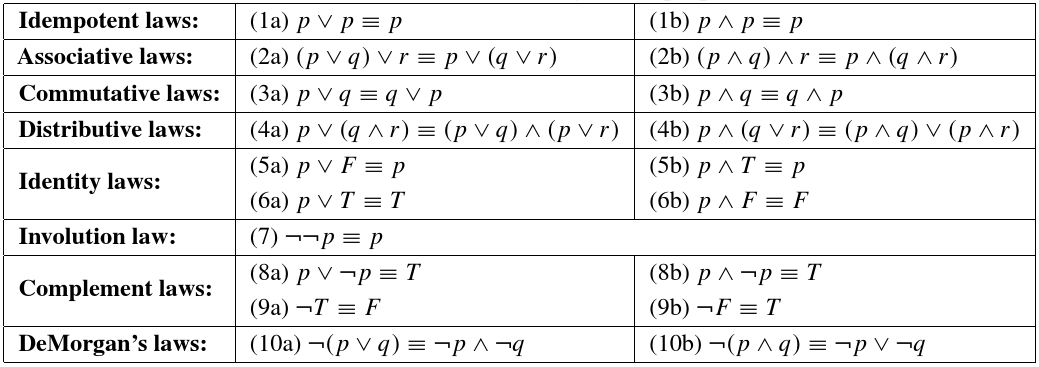
\includegraphics[width=0.7\linewidth]{md/tabla_4-1}
 \caption{Leyes para el álgebra de proposiciones}
\label{fig:tabla:4.1}
\end{figure}



\subsection{Sentencias condicionales y bicondicionales}


 Muchas sentencias, particularmente en matem\'aticas, son de la forma \texttt{``si $p$ entonces $q$''}.  Tales sentencias son llamdas \emph{condicionales} y son denotadas por 
 $$
 p \imply q.
 $$ 



 El condicional $p \imply q$ es frecuentemente le\'ido como \emph{``$p$ implica $q$''} o \emph{``$p$ s\'olo si $q$''.}



 Otra sentencia com\'un es de la forma \emph{``$p$ si y solo si $q$''.}  Tales sentencias son llamadas \emph{bicondicionales} y se denota por 
 $$
 p \iff q.
 $$



 \begin{tdv}[Condicional]
\begin{center}
 \begin{tabular}{|l|l||l|} \hline
$p$ & $q$ & $p \imply q$ \\ \hline
$1$ & $1$ & $1$ \\ \hline
$1$ & $0$ & $0$ \\ \hline
$0$ & $1$ & $1$ \\ \hline
$0$ & $0$ & $1$ \\ \hline
\end{tabular}
\end{center}

 \end{tdv}




 \begin{tdv}[Bicondicional]
\begin{center}
\begin{tabular}{|l|l||l|} \hline
$p$ & $q$ & $p \biconditional q$ \\ \hline
$1$ & $1$ & $1$ \\ \hline
$1$ & $0$ & $0$ \\ \hline
$0$ & $1$ & $0$ \\ \hline
$0$ & $0$ & $1$ \\ \hline
\end{tabular}
\end{center}

 \end{tdv}




 \begin{exmp}
  Demuestre que $$p\imply q \equiv \neg p \vee q.$$
 \end{exmp}




 \begin{exmp} Determine cuales de las siguientes sentencias son tautolog\'ias, construyendo las correspondientes tablas de verdad.
  \begin{enumerate}
   \item $\neg\left( p \vee \neg q \right) \imply \neg p$
   \item $p \imply \left( q\imply r \right)$
   \item $\left( p \imply q \right)\imply r$
   \item $\left( p\imply q \right) \imply \left( q\imply p \right)$
   \item $\left( p \wed \left( p \imply q \right) \right) \imply q$
   \item $\left( p \wed q \right) \imply p$
   \item $q \imply \left( \neg p \vee \neg q \right)$
   \item $\left( \left( p\imply q \right) \wed \left( q \imply r \right) \right) \imply \left( p \imply r \right)$
  \end{enumerate}

 \end{exmp}



\subsection{Argumentos}


 Un \emph{argumento} es una afirmaci\'on de que un conjunto dado de proposiciones $$P_{1}, P_{2},...,P_{n},$$ llamadas \emph{premisas}, tiene como consecuencia otra proposicion $Q,$ llamada \emph{conclusi\'on.}
 
 En otras palabras, es una sentencia de la forma
 $$
  \left( P_{1} \wed P_{2} \wed...\wed P_{n}\right) \imply Q
  $$
 
 
 
 Tal argumento se denota por $$P_{1}, P_{2},...,P_{n} \yields Q.$$



 La noci\'on de \emph{``argumento l\'ogico''} o \emph{``argumento v\'alido''} se formaliza de la manera siguiente:
 
 
 \begin{defn}
  \label{lip:4.4}
  Un argumento $P_{1}, P_{2},...,P_{n} \yields Q$ se dice que es \emph{v\'alido} si la proposici\'on 
  $$
  \left( P_{1} \wed P_{2} \wed...\wed P_{n}\right) \imply Q
  $$ es una tautolog\'ia.
  
   Si un argumento no es \emph{v\'alido,} diremos que es una \emph{falacia.}
 \end{defn}




 \begin{exmp}
 \label{lip:exmp:4.4}
  \begin{enumerate}
   \item Demuestre que $p, p\imply q \yields q$ es un argumento v\'alido. 
   \item Demuestre que $p\imply q, q \yields p$ es una falacia.
   
   \item Demuestre que $p\imply q, \neg q \yields \neg p$ es un argumento v\'alido.
  \end{enumerate}

 \end{exmp}




 \begin{exmp}
  Un principio fundamental del razonamiento l\'ogico nos dice que:
  \begin{center}
   Si $p$ implica $q$ y $q$ implica $r,$ entonces $p$ implica $r.$ 
  \end{center}


En otras palabras, el siguiente argumento es v\'alido
$$
p\imply,q, q\imply r \yields p \imply r.
$$ 
 \end{exmp}

% TODO: \usepackage{graphicx} required
\begin{figure}
	\centering
	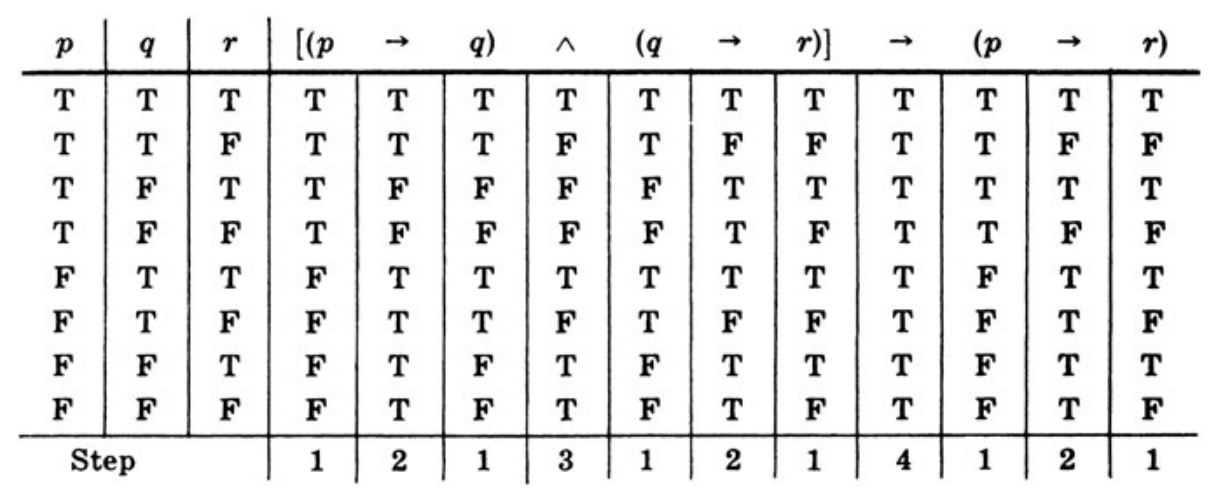
\includegraphics[width=0.7\linewidth]{md/tabla_silogismo}
	\caption{}
	%\label{fig:tablasilogismo}
	\label{fig:tabla_silogismo}
\end{figure}


\begin{exmp}
  \begin{center}
\begin{tabular}{l}
Si sube el d\'olar, sube la gasolina.\\
Si sube la gasolina, entonces hay inflaci\'on.\\\hline
$\therefore$ Si sube el d\'olar, entonces hay inflaci\'on.
 \end{tabular}
 \end{center}
\end{exmp}


\subsection{Funciones proposicionales y Cuantificadores}


 Una \emph{funci\'on proposicional} (o \emph{sentencia abierta} o \emph{condici\'on}) definida en un conjunto $A$ es una expresi\'on $p(x)$ que tiene la propiedad de que $p(a)$ es cierta o falsa para cada $a \in A.$



 El conjunto $A$ se conoce como dominio de $p(x),$ y el subconjunto de todos los elementos para los cuales $p(x)$ es cierto se conoce como el \emph{conjunto de verdad} $T_{p}$ de $p(x):$
 
 $$T_{p}=\set{x \mid x\in A, p(x)=\texttt{1}},$$ 
 o simplemente 
 $$
 T_{p}=\set{x \mid p(x)}.
 $$



 \begin{exmp}
  \label{lip:exmp:4.7}
  Encuentre el conjunto de verdad para cada funci\'on en el conjunto $\N$ de los enteros positivos:
  \begin{enumerate}
   \item $p(x): x+2>7$ 
   \item $p(x): x+5<3$ 
   \item $p(x): x+5>1$ 
  \end{enumerate}

 \end{exmp}



\subsection{Cuantificador universal}


 Sea $p(x)$ una funci\'on proposicional definido en un conjunto $A.$ La expresi\'on
 \begin{equation}
 \label{lip:4.1}
   \forall x \in A: p(x)
 \end{equation}

 
 se lee como  \texttt{``para todo $x\in A,$ $p(x)$ es verdadero.''}  
 
 El s\'imbolo $\forall$ (\texttt{``para todo''}) se llama cuantificador universal.




 Mientras que $p(x)$ es una sentencia abierta (su valor de verdad depende de cada $x\in A$), la afirmaci\'on 
 $$\forall x\in A: p(x)$$ es verdadera si y solo si $p(x)$ se cumple para todo $x\in A.$  



 Por otro lado, si existe alg\'un $x\in A$ tal que $p(x)$ es falso, entonces $$\forall x\in A: p(x)$$ es falso.



 \begin{exmp}
  \label{lip:exmp:4.8}
  Verifique el valor de verdad de las siguientes afirmaciones:
  \begin{enumerate}
   \item $\forall n \in \N: n+4>3.$ 
   \item $\forall n \in \N: n+2>8.$
  \end{enumerate}

 \end{exmp}



\subsection{Cuantificador existencial}


 Sea $p(x)$ una funci\'on proposicional definido en un conjunto $A.$ La expresi\'on
 \begin{equation}
 \label{lip:4.3}
   \exists x \in A: p(x)
 \end{equation} 
 se lee como  \texttt{``existe $x\in A,$ tal que $p(x)$ es verdadero.''}  
 
 El s\'imbolo $\exists$ (\texttt{``existe...''}) se llama cuantificador existencial.




 Mientras que $p(x)$ es una sentencia abierta (su valor de verdad depende de cada $x\in A$), la afirmaci\'on 
 $$\exists x\in A: p(x)$$ es verdadera si y solo si $p(x)$ se cumple alg\'un $x\in A.$  



 Por otro lado, si para todo $x\in A,$ $p(x)$ es falso, entonces $$\exists x\in A: p(x)$$ es falso.



 Verifique el valor de verdad de las siguientes afirmaciones:
 \begin{enumerate}
  \item $\exists n  \in \N: n+4<7;$ 
  \item $\exists n \in \N: n+6<4.$
 \end{enumerate}



\subsection{Negaci\'on de Sentencias Cuantificadas}



 Considere la afirmaci\'on:
 \begin{center}
  \emph{Todos los estudiantes de ingenier\'ia saben programar.}
 \end{center}
?`C\'omo podemos negar esta afirmaci\'on?


\begin{center}
 \emph{Al menos un estudiante de ingenier\'ia no sabe programar.}
\end{center} 



 De manera simb\'olica, si $M$ de ntoa el conjunto de estudiantes de ingenier\'ia, la negaci\'on anterior se puede escribir como
\begin{align*}
  \neg\left( \forall x\in M: \texttt{x sabe programar} \right)\\ \equiv \exists x\in M: \texttt{x no sabe programar.}
\end{align*}




 Si en el ejercicio anterior definimos $$p(x):\texttt{x sabe programar},$$ entonces podemos reescribir la equivalencia anterior como
 \begin{align*}
  \neg\left( \forall x\in M: p(x) \right)\\ \equiv \exists x\in M: \neg p(x).
\end{align*}



 De manera similar
 \begin{center}
  \emph{No hay estudiante de ingenier\'ia que sepa programar}
 \end{center}
 se puede reescribir como
 \begin{center}
  \emph{Cada uno de los estudiantes de ingenier\'ia no saben programar.}
 \end{center}





 De manera simb\'olica, podemos reescribir
  \begin{align*}
  \neg\left( \exists x\in M: p(x) \right)\\ \equiv \forall x\in M: \neg p(x).
\end{align*}



 \begin{thm}[DeMorgan]
  \begin{align}
  \label{lip:thm:4.4}
   \neg\left( \forall x\in M: p(x) \right)& \equiv \exists x\in M: \neg p(x)\\
   \label{lip:thm:4.5}
   \neg\left( \exists x\in M: p(x) \right)& \equiv \forall x\in M: \neg p(x).
  \end{align}

 \end{thm}




 \begin{exmp}
  \label{lip:exmp:4.10.a}
  La negaci\'on de la siguiente afirmaci\'on
  \begin{center}
   \emph{Para todo entero positivo $n,$ tenemos que $n+2>8$}
  \end{center}
es 
\begin{center}
 \emph{Existe un entero positivo $n$ tal que $n+2 \leq 8.$}
\end{center}

 \end{exmp}




 \begin{exmp}
  \label{lip:exmp:4.10.b}
  La negaci\'on de la siguiente afirmaci\'on
  \begin{center}
   \emph{Existe una persona viva con 150 a\~nos o m\'as.}
  \end{center}
 es 
 \begin{center}
  \emph{Toda persona viva tiene menos de 150 a\~nos.}
 \end{center}

 \end{exmp}




 \begin{rem}
  Para negar una afirmaci\'on del tipo $$\forall x \in A: p(x)$$ s\'olo necesitamos encontrar un elemento $x_{0}\in A$ tal que $p(x)$ sea \emph{falso.}
  
  
  A un elemento $x_{0}$ as\'i se le conoce como \emph{contraejemeplo.}
 \end{rem}




 \begin{exmp}
 \label{lip:4.11}
  \begin{enumerate}[(a)]
   \item 
  Un contraejemplo para $\forall x \in \R: \abs{x}\neq 0$ es $x=0.$  
   \item 
  Un contraejemplo para $\forall x \in \R: x^{2}\geq x$ es $x=\frac{1}{2}.$  
   \item 
  Sin embargo, $\forall x \in \N: : x^{2}\leq x$ es siempre cierto.
  \end{enumerate}

 \end{exmp}



\subsection{Ejemplos Resueltos}

\subsection{Proposiones y Tablas de Verdad}


 \begin{exmp}
  Sea $p:\texttt{``Hace fr\'io''}$ y $q:\texttt{``Est\'a lloviendo''.}$ Proponga un enunciado verbal simple que describa cada una de las siguientes proposiciones:
  \begin{enumerate}
   \item $\neg p;$
   \item $p \wed q;$
   \item $p \vee q;$
   \item $q \vee \neg p.$
  \end{enumerate}

 \end{exmp}




 \begin{exmp}
  Encuentre la tabla de verdad de $\neg p \wed q.$
 \end{exmp}




 \begin{exmp}
  Demuestre que la propisici\'on 
  $$
  p \vee \neg \left( p\wed q \right)
  $$ es una tautolog\'ia.
 \end{exmp}




 \begin{exmp}
  Muestre que las proposiciones $\neg\left( p \wed q \right)$ y $\neg p \vee \neg q$ son l\'ogicamente equivalentes.
 \end{exmp}




 \begin{exmp}
  Use las leyes en la tabla \ref{fig:tabla:4.1} para mostrar que 
  $$
  \neg \left( p \wed q \right) \vee \left( \neg p \wed  q \right) \equiv \neg p
  $$
 \end{exmp}



\subsection{Sentencias condicionales}


 \begin{exmp}
  \label{lip:sol:4.6}
  Reescriba los siguientes enunciados sin usar el condicional:
  \begin{enumerate}
   \item Si hace fr\'io, el usa sombrero. 
   \item Si la productividad se incrementa, entonces el salario aumenta.
  \end{enumerate}

 \end{exmp}




 \begin{exmp}
  \label{lip:sol:4.7}
  Considere la proposici\'on condicional $p \imply q.$ La proposiones 
  \begin{center}
  ${\color{red}q \imply p,} {\color{blue}\, \neg p \imply \neg q,} \, {\color{green}\neg q \imply \neg p}$
  \end{center}
son llamadas {\color{red} conversa,} {\color{blue}inversa} y {\color{green} contrapositiva}, respectivamente.


?`Cu\'ales de estas proposiciones son l\'ogicamente equivalente s a $p\imply q$?
 \end{exmp}




 \begin{exmp}
  Determine la contrapositiva de cada enunciado:
  \begin{enumerate}
   \item Si Erik es poeta, entonces es pobre. 
   \item Solo si Marcos estudia, pasar\'a el examen. 
  \end{enumerate}

 \end{exmp}




 \begin{exmp}
  Escriba la negaci\'on de cada enunciado, tan simple como sea posible:
  \begin{enumerate}
   \item Si ella trabaja, ganar\'a dinero. 
   \item El nada si y solo si el agua est\'a tibia. 
   \item Si neva, entonce no manejar\'e.
  \end{enumerate}

 \end{exmp}



\subsection{Argumentos}


 \begin{exmp}
  Muestre que el siguiente argumento es una falacia:
 $$
 p\imply q, \neg p \yields \neg q.
 $$
 \end{exmp}




 \begin{exmp}
  Muestre que el siguiente argumento es v\'alido:
 $$
 p\imply q, \neg q \yields \neg p.
 $$
 \end{exmp}




\begin{exmp}
  Muestre que el siguiente argumentos siempre es v\'alido:
 $$
 p \imply \neg q, r \imply q, r \yields \neg p.
 $$
\end{exmp}




 \begin{exmp}
  Determine la validez del siguiente argumento:
  \begin{center}
\begin{tabular}{l}
Si $7$ es menor que $4$, entonces $7$ no es n\'umero primo\\
$7$ no es menor que $4$\\\hline
$7$ no es n\'umero primo.
  \end{tabular}
  \end{center}

 \end{exmp}




 \begin{exmp}
  Determine la validez del siguiente argumento:
  \begin{center}
\begin{tabular}{l}
Si dos lados de un tri\'angulo son iguales, entonces los respectivos \'angulos opuestos son iguales\\
Dos lados de un tri\'angulo no son iguales\\\hline
Los respectivos \'angulos opuestos no son iguales.
  \end{tabular}
  \end{center}

 \end{exmp}



\subsection{Cuantificadores y Funciones Proposicionales}


 \begin{exmp}
  Sea $A=\set{1,2,3,4,5}.$ Determine el valor de verdad de cada uno de los siguientes enunciados:
  \begin{enumerate}
   \item $\exists x \in A: x+3=10;$ 
   \item $\forall x \in A: x+3<10;$ 
   \item $\exists x \in A: x+3<5;$ 
   \item $\forall x \in A: x+3 \leq 7.$
  \end{enumerate}

 \end{exmp}




  \begin{exmp}
    Determine el valor de verdad de cada uno de las siguientes afirmaciones donde $U=\set{1,2,3}$ es el conjunto \emph{``universo''} (de referencia):
 \begin{enumerate}
  \item $\exists x \forall y: x^{2}< y+1;$ 
  \item $\forall x \exists y: x^{2}+y^{2}<12;$ 
  \item $\forall x \forall y: x^{2}+y^{3}<12.$
 \end{enumerate}

  \end{exmp}




 \begin{exmp}
  Encuentre la negaci\'on de cada una de las siguientes afirmaciones:
  \begin{enumerate}
   \item $\exists x \forall y: p(x,y);$ 
   \item $\forall x \forall y: p(x,y);$ 
   \item $\exists x \exists y \forall z: p(x,y,z).$
  \end{enumerate}

 \end{exmp}




 \begin{exmp}
  Sea $$p(x): x+2>5.$$ Indique cuando $p(x)$ es una funci\'on proposicional o no en cada uno de los siguientes conjuntos: 
  \begin{enumerate}
   \item $\N$ 
   \item $\Z^{-}=\set{-1,-2,-3,...}$ 
   \item $\mathbb{C}$
  \end{enumerate}

 \end{exmp}




	\begin{exmp}
	Niegue cada uno de las siguientes afirmaciones:
	\begin{enumerate}
		\item Todos los estudiantes viven en los dormitorios.
		\item A todos los estudiantes de ingeniería le gusta el futbol.
		\item Algunos estudiantes tienen 25 años o más.
	\end{enumerate}
	\end{exmp}



 \subsection{Bibliograf\'ia}
 Las notas de esta secci\'on est\'an basadas en el cap\'itulo 4 \texttt{``Logic and Propositional Calculus''} del libro
 \begin{center}
  \texttt{Lipschutz, S. and Lipson, M.;\textbf{ Schaum's Outline of Discrete Mathematics;} McGraw-Hill, 3th Edition.}
 \end{center}

\section{Teoría de Conjuntos}

\subsection{Conjuntos y Elementos. Subconjuntos}


	Un \emph{conjunto} puede ser visto como un conjunto bien definido de objetos, llamados \emph{elementos} o \emph{miembros} de tal conjunto. 
	
	Usualmente, usaremos letras mayúsculas para denotar conjunto, y minúsculas para dlos elementos. 



	La pertenencia en un conjunto se denota de la siguiente manera:
	\begin{center}
		\emph{$a \in S$ denota que $a$ pertenece al conjunto $S.$} 
		
		\emph{$a,b \in S$ denota que tanto $a$ como $b$ pertenecen al conjunto $S.$}
	\end{center}
	
	El símbolo $\in$ significa \texttt{``es elemento de''.}  Por el contrario, $\notin$ significa \texttt{``no es elemento de''.}


\subsection{Especificación de Conjuntos}


	Básicamente, existen dos maneras de especificar un conjunto en particular.  Por un lado, si es posible, enlistar todos los miembros.  Por otro lado, caracterizando los elementos en el conjunto.



	En cualquier caso, para declarar un conjunto se utilizan llaves:
	$$
	A=\set{\cdots}
	$$



	Por ejemplo, el conjunto 
	$$
	A=\set{1,3,5,6,9}
	$$
	tambi\'en se puede especificar como
	$$
	A=\set{x\in \N \mid x<10, 2\nmid x }
	$$



	Un conjunto no depende del modo en que sus elementos se muestren.  Este permanece igual si sus elementos se repiten o se reacomodan.




	\begin{problema}
		\begin{align}
			\set{x\in\R | x^{2}-3x+2=0} & =\set{1,2} \\
			&=\set{1,2,2,1}
		\end{align}
		
	\end{problema}
	


\subsection{Subconjuntos}


	Supongamos que cada elemento en un conjunto $A$ es tambi\'en elemento del conjunto $B,$ es decir,
	$$
	x\in A \onlyif x\in B.
	$$



	En ese caso, decimos que $A$ es subconjunto de $B.$  Tambi\'en podemos decir que $A$ está contenido en $B$ o que $B$ contiene a $A$.



	Esta relación se escribe como
	$$
	A \subset B 
	$$ o en ocasiones como
	$B\supset A.$  Por el contrario, si es necesario indicar que $A$ \emph{no} es  subconjunto de $B,$ escribimos $A \not\subset B.$



	Diremos que dos conjuntos son iguales si poseen los mismos elementos, es decir, 
	$$
	x \in A \iff x \in B.
	$$



	De manera equivalente 
	\begin{center}
		$A=B$ si y solo si $A \subset B$ y $B \subset A.$
	\end{center}
	



	\begin{problema}
		\label{lip:exmp:1.2}
		Determine la relación entre los siguientes conjuntos
		\begin{center}
			$$A=\set{1,3,4,7,8,9}, \, 
			B=\set{1,2,3,4,5}, \,
			C=\set{1,3}.$$
		\end{center}
		
	\end{problema}
	



	\begin{problema}
		Demuestre que 
		\begin{enumerate}
			\item $A\not\subset B$ si y solo $\exists x\in A: x\notin B.$
			\item $A \subset A.$
			\item $A\subset B, B\subset C \onlyif  A\subset C.$
		\end{enumerate}
		
	\end{problema}
	


\subsection{Símbolos especiales}

 Algunos conjuntos num\'ericos tienen una notación especial
	\begin{itemize}
		\item $\N:$ números naturales (enteros positivos); 
		\item $\Z:$ números enteros; 
		\item $\Q:$ números racionales; 
		\item $\R:$ números reales; 
		\item $\mathbb{C}:$ números complejos.
	\end{itemize}
	
	



	Observe que
	$$
	\N \subset \Z \subset \Q \subset \R \subset \mathbb{C},
	$$ pero en ningún caso los conjuntos son iguales. 


\subsection{Conjunto Universal y Conjunto Vacío}


	Todos los conjuntos bajo investigación en una apliación de teoría de conjuntos se supone que pertenecen a un conjunto fijo más grande llamado \emph{conjunto universo} $\uset,$ al menos que se indique otro caso.



	Dado un conjunto universal $\uset$ y una propiedad $P,$ es posible que no existan elemento de $\uset$ con la propiedad $P.$ 



	Por ejemplo, el siguiente conjunto no tiene elementos
	$$
	S=\set{x\in \Z \mid x^{2}=3}.
	$$



	A tal conjunto sin elementos $\set{}$ se le conoce como conjunto vacío y se denota como $\emptyset.$



	\begin{rem}
		\emph{Sólo existe un conjunto vacío}.  El conjunto vacío es subconjunto de cualquier otro conjunto.
	\end{rem}
	


\subsection{Conjuntos disjuntos}


	Dos conjuntos $A$ y $B$ son \emph{disjuntos} si no tienen elementos en común. 



	\begin{problema}
		Considere $$
		A=\set{1,2}, \; B=\set{4,5,6}, \; C=\set{5,6,7,8}.
		$$
		Determine que pares de conjuntos son disjuntos. 
	\end{problema}
	


\subsection{Diagramas de Venn}


	Un diagrama de Venn es una representación gráfica de conjuntos en el que cada conjunto está representado por áreas encerradas en el plano.



	El conjunto universo $\uset$ es representado por el interior de un rectángulo, y cualquier otro conjunto esta representado por discos que viven dentro del rectángulo.



	\begin{figure}
		\centering
		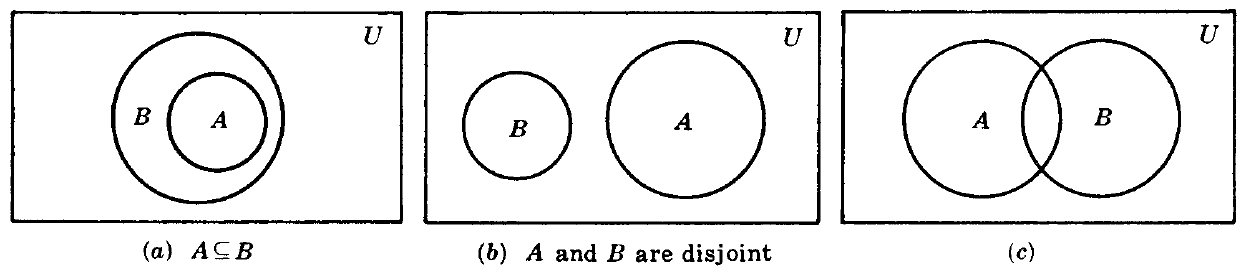
\includegraphics[width=11cm,keepaspectratio=true]{./md/venn01.png}
		% venn01.png: 0x0 pixel, 300dpi, 0.00x0.00 cm, bb=
		\caption{Representaciones con Diagramas de Venn}
		\label{fig:0101}
	\end{figure}
	


\subsection{Operaciones con Conjuntos}


	En esta sección introduciremos la unión, la intersección y el complemento de conjuntos.


\subsection{Unión e Intersección}


	La unión de dos conjuntos $A$ y $B$ es el conjunto de todos los elementos que pertenecen a $A$ o a $B,$  es decir
	$$
	A \cup B = \set{x \mid x\in A \vee x\in B}.
	$$



	La intersección de dos conjuntos $A$ y $B$ es el conjunto de todos los elementos que pertenecen a $A$ y a $B,$  es decir
	$$
	A \cap B = \set{x \mid x\in A \wed x\in B}.
	$$



	\begin{figure}
		\centering
		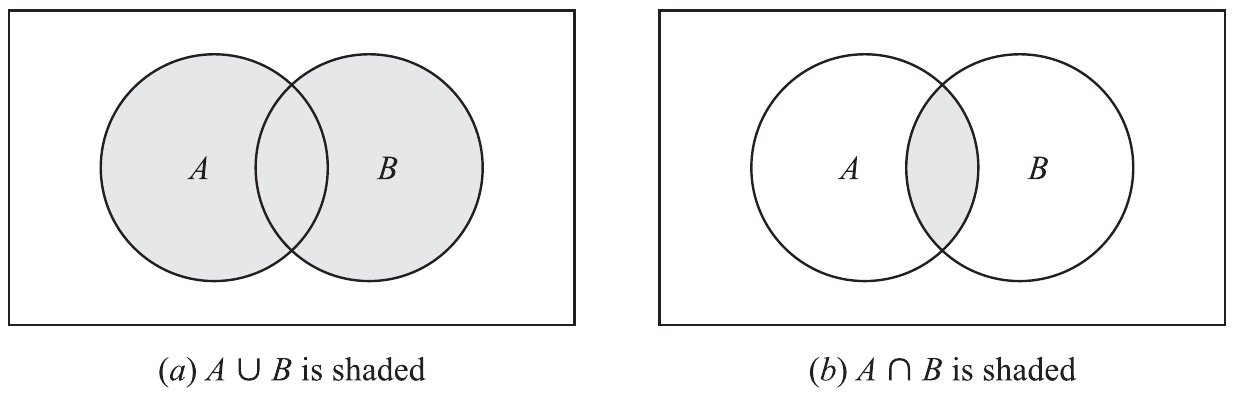
\includegraphics[width=10cm,keepaspectratio=true]{./md/venn_union_interseccion.png}
		% venn_union_interseccion.png: 0x0 pixel, 300dpi, 0.00x0.00 cm, bb=
		\caption{Unión e Intersección}
		\label{fig:0103}
	\end{figure}
	




	\begin{problema}
		\label{lip:exmp:1.4.a}
		Sea $A=\set{1,2,3,4},$ $B=\set{3,4,5,6,7},$ $C=\set{2,3,8,9}.$ Encuentre 
		\begin{enumerate}
			\item $A \cup B=$ 
			\item $A \cap B=$ 
			\item $A \cup C=$ 
			\item $A \cap C=$ 
			\item $B \cup C=$ 
			\item $B \cap C=$
		\end{enumerate}
		
	\end{problema}
	



	\begin{problema}
		\label{thm:1.3}
		Demuestre que para cualesquiera dos conjuntos $A$ y $B,$ tenemos:
		$$
		A \cap B \subset A \subset A \cup B.
		$$
	\end{problema}
	



	\begin{problema}
		\label{thm:1.4}
		Demuestre que las siguientes proposiciones son equivalentes:
		\begin{enumerate}
			\item $\displaystyle A \subset B$
			\item $\displaystyle A \cap B = A$
			\item $\displaystyle A \cup B = B$
		\end{enumerate}
		
	\end{problema}
	



	Dos conjuntos $A$ y $B$ se dicen \emph{disjuntos} si no tienen elementos en común, es decir $A\cap B=\emptyset$.
	
	
	Supongamos que 
	$$
	S=A\cup B, \; A\cap B=\emptyset.
	$$  Diremos que $S$ es la unión disjunta de $A$ y $B$ y se denota por $$S=A \sqcup B.$$ 
	


\subsection{Complementos, Diferencias y Diferencias Sim\'etricas}


	En esta sección, consideraremos conjuntos que sean subconjuntos de un conjunto universo fijo $\uset.$



	El \emph{complemento} $A^{C}$ de un conjunto $A$ es el conjunto de elementos que no pertenecen a $A$, es decir 
	$$A^{C}=\set{x\in \uset \mid x \notin A}.$$



	Algunos textos denotan $A^{C}$ tambi\'en como $A'$ o $\bar{A}.$ 



	El \emph{complemento relativo} de un conjunto $B$ con respecto a un conjunto $A$ se define como 
	$$
	A\minus B = \set{x \mid x \in A, x \notin B}.
	$$


% 
%  \begin{problema}
%   Demuestre que 
%   $A \minus B = A \cap B^{C}$
%  \end{problema}
% 
% 



	El conjunto $A\minus B$ se lee \texttt{$A$ menos $B$.} Algunos textos lo denotan tambi\'en como $A-B.$  



	La \emph{diferencia sim\'etrica} de los conjuntos $A$ y $B$ se define como $$A\symdif B=\left( A\cup B \right)\minus \left( A \cap B \right).$$



	\begin{figure}
		\centering
		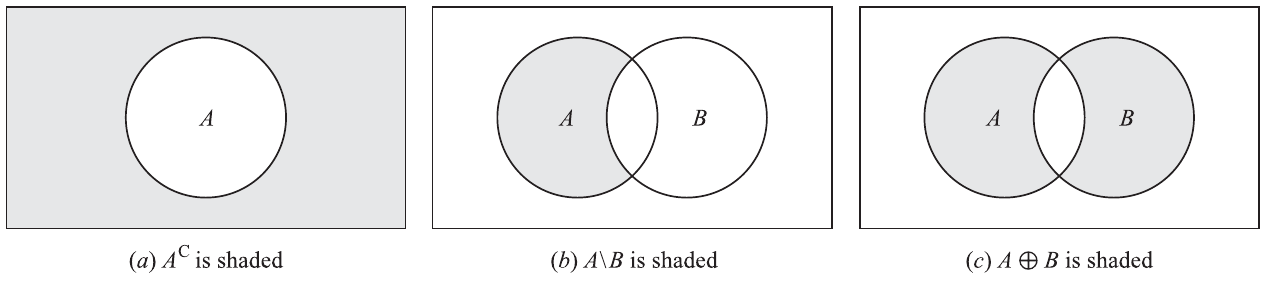
\includegraphics[width=10cm,keepaspectratio=true]{./md/venn_complemento.png}
		% venn_complemento.png: 0x0 pixel, 300dpi, 0.00x0.00 cm, bb=
		\caption{Complementos, diferencia y diferencia simétrica.}
		\label{fig:0104}
	\end{figure}
	




\begin{problema}
Definamos $$p\veebar q \equiv \left( p \vee q \right) \wed \neg\left( p \wed q \right)$$
Demuestre que 
\begin{enumerate}
\item $ \displaystyle
x \in A\symdif B \iff \left( x \in A \right) \veebar \left( x \in B  \right)
$ 
\item $\displaystyle p\veebar q \equiv \left( p \wed \neg q \right) \vee \left( q \wed \neg p \right)$ 
\item $\displaystyle A \veebar B = \left( A \minus B \right) \cup \left( B \minus A \right)$
\end{enumerate}

\end{problema}




\begin{problema}
\label{lip:exmp:1.5}
Supongamos que $\N$ es el conjunto universo. Definamos $A=\set{1,2,3,4},$ $B=\set{3,4,5,6,7},$ $C=\set{2,3,8,9},$ $E=\set{2,4,6,...}.$

Determine:
\begin{enumerate}
\item $A \symdif B$ 
\item $A \symdif C$ 
\item $B \symdif C$ 
\item $A \symdif E$
\end{enumerate}
\end{problema}



\subsection{Conjuntos fundamentales}


Dos conjuntos $A$ y $B$ se dicen \emph{disjuntos} si no tienen elementos en común, es decir $A\cap B=\emptyset$.


Supongamos que 
$$
S=A\cup B, \; A\cap B=\emptyset.
$$  Diremos que $S$ es la unión disjunta de $A$ y $B$ y se denota por $$S=A \sqcup B.$$ 




En general $S$ es una unión disjunta de $P_{1}, P_{2},...,P_{n}$ si 
\begin{itemize}
\item $\displaystyle S=P_{1}\cup P_{2}\cup...\cup P_{n}$ y
\item $P_{i}\cap P_{j}=\emptyset$ siempre y cuando $i\neq j.$
\end{itemize}


En este caso, escribimos
$$
S=P_{1}\sqcup P_{2}\sqcup...\sqcup P_{n}.
$$



Diremos que $P_{1}, P_{2},...,P_{n}$ es sistema de conjuntos fundamentales para $\uset$ si
$$
\uset = P_{1}\sqcup P_{2}\sqcup...\sqcup P_{n}.
$$



\begin{problema}
\label{lip:exmo:1.6}
Contruya un sistema de conjuntos fundamentales a partir de tres conjunto $A, B, C.$  
\end{problema}



\begin{figure}
\centering
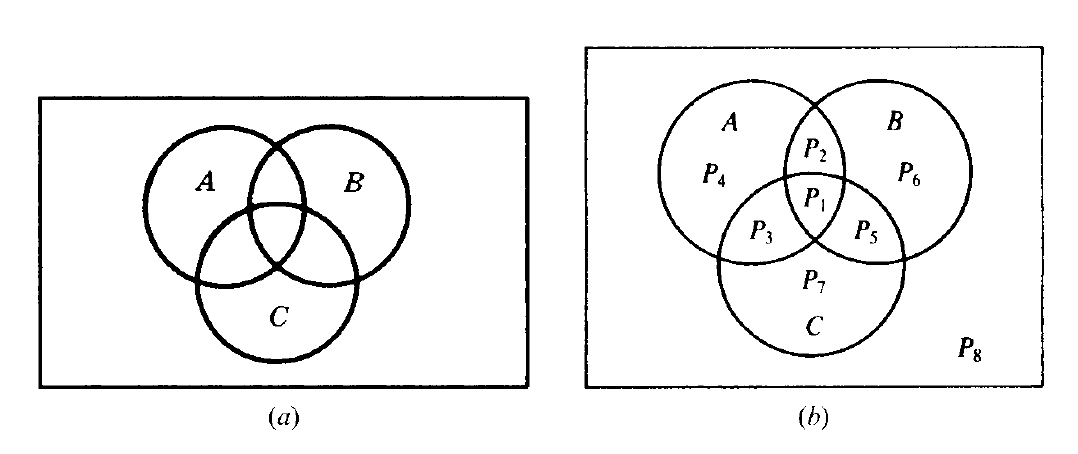
\includegraphics[width=10cm,keepaspectratio=true]{./md/sistema_fundamental.png}
% sistema_fundamental.png: 0x0 pixel, 300dpi, 0.00x0.00 cm, bb=
\label{fig:0105}
\end{figure}




\subsection{Álgebra de conjuntos, dualidad}


	Los conjuntos bajo las operaciones de unión, intersección y complemento satisface varias leyes o identidad, que se enuncian en la siguiente tabla, y son similares a las leyes de lógica.



	\begin{figure}
		\centering
		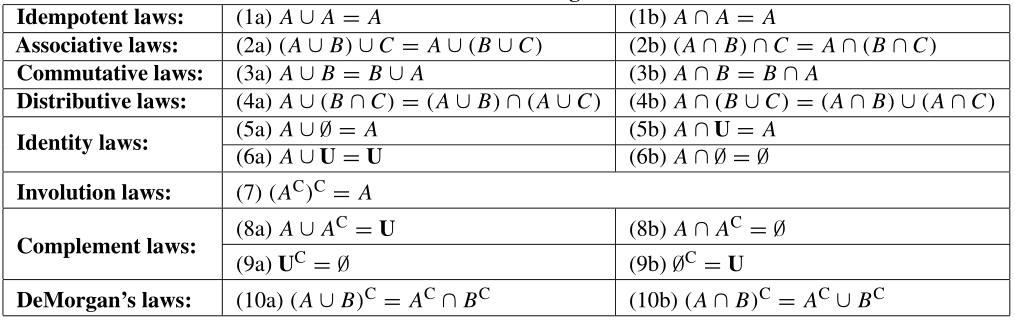
\includegraphics[width=11cm,keepaspectratio=true]{./md/leyes_conjuntos.png}
		\caption{Leyes de Conjuntos}
		\label{fig:leyesconjuntos}
	\end{figure}
	



	Cada ley de conjuntos se corresponde con una ley de lógica. Por ejemplo, la ley de DeMorgan:
	\begin{align*}
		\left(A \cup B\right)^{C} &= \set{x \mid x\notin(A \cup B)}\\
		&= \set{x \mid x\notin A \wed x\notin B}\\
		&=A^{C}\cap B^{C}
	\end{align*}



	{Dualidad}
	El \emph{principio de dualidad} establece que la equivalencia $E^{*}$ obtenida a partir de una ley de lógica $E$ reemplazando
	\[ \cup, \cap, \uset, \emptyset\] por
	\[ \cap, \cup, \emptyset, \uset\]
	sigue siendo una ley de lógica.
	
	
	A la proposición $E^{*}$ se le conoce como dual $E.$



	\begin{problema}
		Encuentre el dual de 
		\[ (\uset \cap A) \cup (B\cap A) = A\]
	\end{problema}



\section{Inducci\'on Matem\'atica}

\subsection{Introducci\'on}


	Una propiedad esencial de los naturales $\N=\set{1,2,3,...}$  es la siguiente
	
	
	\begin{ax}[Principio de Inducci\'on Matem\'atica, versi\'on I]
		Sea $P$ una proposici\'on definida en $\N,$ es decir, $P(n)$ toma valores de cierto o falso para cada $n\in \N.$
		
		Supongamos que
		\begin{enumerate}
			\item $P(1)$ es cierto;
			\item $\forall k \in \N: P(k) \onlyif P(k+1).$
		\end{enumerate}
		
		Entonces $P$ es {cierto} para todo entero positivo $n\in \N.$
	\end{ax}
	


[t]
	\begin{exmp}
		Sea $P(n):1+3+5+...+(2n-1)=n^2.$ Demostrar que $P(n)$ es cierta para toda $n \in \N.$ 
	\end{exmp}



	\begin{ax}[Principio de Inducci\'on Matem\'atica, versi\'on II]
		Sea $P$ una proposici\'on definida en $\N$ tal que :
		\begin{enumerate}
			\item $P(1)$ es cierta;
			\item $P(k)$ es cierta siempre que $P(j)$ para toda $1\leq j < k.$
		\end{enumerate}
		Entonces $P(n)$ es cierta para toda $n\in \N.$
	\end{ax}
	



	\begin{rem}
		Algunas veces, uno desea demostrar que una proposici\'on es cierta para alg\'un conjunto de enteros
		$$
		\set{a,a+1, a+2,...}
		$$
		donde $a$ es un entero positivo, posiblemente cero. Esto puede hacerse simplemente reemplazando $1$ por $a$ en cualquier versi\'on del Principio de Inducci\'on Matem\'atica. 
	\end{rem}
	


\subsection{Notaci\'on ``Sigma''}


	La letra griega $\Sigma$ denota adici\'on repetida:
	
	$$
	\sum_{i=a}^{b} f(i)=f(a)+f(a+1)+...+f(b),
	$$ siempre que $a\leq b.$



	\begin{exmp}
		\label{ayr:exmp23.1}
		\begin{enumerate}
			\item $\sum_{j=1}^{5} j = 1+2+3+4+5 =15$
			\item $\sum_{i=0}^{3} \left( 2i+1 \right)=
			1+3+5+7$
			\item $\sum_{i=2}^{10} i^{2}=2^{2}+3^{2}+...+10^{2}$
			\item $\sum_{j=1}^{4}\cos(j\pi)=
			\cos\pi+ \cos 2\pi + \cos 3\pi +\cos 4\pi.$
		\end{enumerate}
		
	\end{exmp}
	



	{Linealidad}
	\begin{prop}
		\label{suma:linealidad}
		\begin{align}
			\sum_{i=a}^{b} cf(i)&=c \sum_{i=a}^{b} f(i)\\
			\sum_{i=a}^{b} f(i)+g(i)&= \sum_{i=a}^{b} f(i)
			+\sum_{i=a}^{b} g(i)
		\end{align}
		
	\end{prop}
	



	{Propiedades}
	\begin{align}
		\sum_{k=a}^{b}f(k)&=\sum_{j=a}^{b}f(j)\\
		\sum_{j=a}^{a}f(j)&=f(a) \\
		\sum_{j=a}^{c}f(j)&=\sum_{j=a}^{b}f(j)+\sum_{j=b}^{c}f(j) \\
		\sum_{j=a}^{b+1}f(j)&=\sum_{j=a}^{b}f(j)+f(b)
	\end{align}
	



	\begin{exmp}
		Si $f(n)=(2n-1),$ entonces
		$$
		\sum_{i=1}^{n}f(j)=1+3+...+\left( 2n-1 \right)
		$$ es la suma hasta el $n-$\'esimo natural impar.  Observe que 
		\begin{enumerate}
			\item $\sum_{j=1}^{1}f(j)=2(1)-1=1.$
			\item $\sum_{i=1}^{n+1}f(j)=\left( \sum_{i=1}^{n}f(j) \right)+\left( 2n+1 \right)$
		\end{enumerate}
		
	\end{exmp}
	



	\begin{exmp}
		Si $f(n)=2^{n-1},$ entonces
		$$
		\sum_{i=1}^{n}f(j)=1+2+...+2^{n-1}
		$$ es la suma de las primeras $n$ potencias de 2 (incluyendo $1=2^{0}$).  Observe que 
		\begin{enumerate}
			\item $\sum_{i=1}^{n+1}f(j)=1+2+...+2^{n}$
			\item $\sum_{j=1}^{1}f(j)=2^{1-1}=1.$
			\item $\sum_{i=1}^{n+1}f(j)=\left( \sum_{i=1}^{n}f(j) \right)+2^{n}.$
		\end{enumerate}
		
	\end{exmp}
	


\subsection{Ejemplos Resueltos}

[t]
	\begin{exmp}
		Demostrar que $$P(n): 1+2+3+...+n=\frac{1}{2}n\left( n+1 \right)$$
		es cierto para todo $n \in \N.$
	\end{exmp}
	


[t]
	\begin{exmp}
		Demostrar que $$P(n): 1+2+2^{2}+...+2^{n}=2^{n+1}-1$$
		es cierto para todo $n \in \N.$
	\end{exmp}
	


\subsection{Funciones definidas de manera recursiva}


	Decimos que una funci\'on est\'a \emph{definida recursivamente} si la definici\'on de la funci\'on se refiere a s\'i misma.



	Para que la funci\'on est\'e bien definida, debe tener las siguientes dos propiedades:
	\begin{enumerate}
		\item Deben existir ciertos argumentos, llamados \emph{valores base,} para los cuales la funci\'on no se refiera a s\'i misma.
		\item Cada vez que la funci\'on se refiera a s\'i misma, el argumento de la funci\'on debe est\'ar m\'as cercano a un valor base.
	\end{enumerate}
	


\subsection{La funci\'on factorial}


	El producto de enteros positivos de $1$ hasta $n$ (inclu\'ido) es llamado \emph{$n$ factorial, $n!$}
	
	Es decir, 
	$$
	n!=n(n-1)\cdots 3\cdot 2 \cdot 1.$$
	



	Por razones combinatorias, es conveniente definir \emph{$0!=1,$} y de esta manera la funci\'on factorial quedar\'a definida para todos los enteros no negativos.


[t]
	\begin{rem}
		\begin{enumerate}
			\item $1!=1\cdot0!$
			\item $2!=2\cdot1!$
			\item $3!=3\cdot2!$
			\item $4!=4\cdot3!$
		\end{enumerate}
		
	\end{rem}
	



	Es f\'acil observar que para $n \in \N:$
	$$
	n!=n\cdot (n-1)!
	$$



	\begin{defn}[Funci\'on factorial]
		$$n!=
		\begin{cases}
			1 & n=0 \\
			n\cdot(n-1)! & n>0
		\end{cases}
		$$
	\end{defn}
	



	\begin{rem}
		\begin{enumerate}
			\item El valor de $n!$ factorial esta dado explicitamente para $n=0,$ de manera que $0$ es el valor base. 
			\item El valor de $n!, n>0$ est\'a dado en t\'erminos de $n-1,$ que es m\'as cercano al valor base $0.$    
		\end{enumerate}
		
		Por tanto, $n!$ es una funci\'on recursiva bien definida.
	\end{rem}
	


[fragile]
	{Implentaci\'on iterativa del \emph{factorial} en \texttt{Python}}
	\begin{verbatim}
		def factorial(n):
		result = 1
		for i in range(1, n+1):
		result *= i
		return result
	\end{verbatim} 


[fragile]
	{Implentaci\'on recursiva del \emph{factorial} en \texttt{Python}}
	\begin{verbatim}
		def factorial(n):
		z=1
		if n>1:
		z=n*factorial(n-1)
		return z
	\end{verbatim}
	Para m\'as implementaciones, visite \href{https://rosettacode.org/wiki/Factorial}{rosettacode.org/wiki/Factorial}



\subsection{Suceci\'on de Fibonacci}


	La celebre sucesi\'on de Fibonacci (usualmente denotada por $F_{0}, F_{1}, F_{2},...$) es como sigue:
	$$
	0,0,1,2,3,5,8,13,21,34,55,...
	$$
	
	Es decir, $F_{0}=0$  $F_{1}=1$ y cada t\'ermino sucesor es la suma de los dos precedentes.



	Por ejemplo, los siguientes dos t\'erminos de la sucesi\'on son
	$$34+55=89 \texttt{ y }55+89=144.$$



	\begin{defn}[Sucesi\'on de Fibonacci]
		$$
		F_{n}=
		\begin{cases}
			n & n=0,1 \\
			F_{n}=F_{n-2}+F_{n-1} & n>1
		\end{cases}
		$$
	\end{defn}



	Este ejemplo es una funci\'on recursiva bien definida, ya que la funci\'on hace referencia a s\'i misma, cuando se usan $ F_{n-2}$ y $F_{n-1},$ y
	\begin{enumerate}
		\item los valores base son $0$ y $1;$
		\item los valores de $F_{n}$ est\'an definidos en t\'erminos de valores m\'as peque\~nos $n-2$ y $n-1$ que son m\'as cercanos a los valores base.
	\end{enumerate}
	


[fragile]
	{Implentaci\'on iterativa de \emph{Fibonacci} en \texttt{Python}}
	\begin{verbatim}
		def fibIter(n):
		if n < 2:
		return n
		fibPrev = 1
		fib = 1
		for num in xrange(2, n):
		fibPrev, fib = fib, fib + fibPrev
		return fib
	\end{verbatim} 


[fragile]
	{Implentaci\'on recursiva de \emph{Fibonacci} en \texttt{Python}}
	\begin{verbatim}
		def fibRec(n):
		if n < 2:
		return n
		else:
		return fibRec(n-1) + fibRec(n-2)
	\end{verbatim}
	Para m\'as implementaciones, visite \href{http://rosettacode.org/wiki/Fibonacci\_sequence}{rosettacode.org/wiki/Fibonacci\_sequence}


\subsection{La funci\'on de Ackermann}


	\begin{defn}[Funci\'on (fallida) de Ackermann]
		$$
		A(m,n)=
		\begin{cases}
			n+1 & m=0\\
			A(m-1,n) & m\neq0, n=0 \\
			A(m-1, A(m,n-1)) & m\neq 0, n\neq 0
		\end{cases}
		$$
	\end{defn}
	



	\begin{defn}[Funci\'on de Ackermann]
		$$
		A(m,n)=
		\begin{cases}
			n+1 & m=0\\
			A(m-1,1) & m\neq0, n=0 \\
			A(m-1, A(m,n-1)) & m\neq 0, n\neq 0
		\end{cases}
		$$
	\end{defn}
	


[fragile]
	{Implentaci\'on recursiva de \emph{Ackermann} en \texttt{Python}}
	\begin{verbatim}
		def ack2(M, N):
		if M == 0:
		return N + 1
		elif N == 0:
		return ack2(M - 1, 1)
		else:
		return ack2(M - 1, ack2(M, N - 1))
	\end{verbatim}
	Para m\'as implementaciones, visite \href{http://rosettacode.org/wiki/Ackermann\_function}{rosettacode.org/wiki/Ackermann\_function}


\subsection{Ejemplos Resueltos}


	\begin{exmp}
		Sean $a,b$ enteros positivos, y definamos la siguiente funci\'on de manera recursiva:
		$$
		Q(a,b)=
		\begin{cases}
			0 & a<b \\
			Q(a-b,b)+1 & b \leq a
		\end{cases}
		$$
		\begin{enumerate}
			\item Encuentre (i) $Q(2,5);$ (ii) $Q(12,5)$
			\item ?`Qu\'e es lo que hace esta funci\'on? Encuentre $Q(5861,7)$
		\end{enumerate}
	\end{exmp}



	\begin{exmp}
		Use la definici\'on de la funci\'on de Ackermann para calcular $A(1,3).$
	\end{exmp}


\subsection{Ejemplos}


	\begin{exmp}
		Demuestre por inducción que 
		$\displaystyle 2+4+6+...+2n=n(n+1)$
	\end{exmp}



	\begin{exmp}
		Demuestre por inducción que 
		$\displaystyle 1+4+7+...+\left( 3n-2 \right)=\dfrac{n\left( 3n-1 \right)}{2}$
	\end{exmp}



	\begin{exmp}
		Demuestre por inducción que 
		$\displaystyle 1^{2}+2^{2}+...+n^{2}=\dfrac{n(n+1)(2n+1)}{6}$
	\end{exmp}



	\begin{exmp}
		Demuestre por inducción que 
		$\displaystyle \dfrac{1}{1\cdot 3}+\dfrac{1}{3\cdot 5}+...+\dfrac{1}{\left( 2n-1 \right)\cdot \left( 2n+1 \right)}=\dfrac{n}{2n+1}$
	\end{exmp}



	\begin{exmp}
		Demuestre por inducción que 		
		$\displaystyle \dfrac{1}{1\cdot 5}+ \dfrac{1}{5 \cdot 9}+...+\dfrac{1}{(4n-3)\cdot (4n+1)}=\dfrac{n}{4n+1}$
	\end{exmp}



	\begin{exmp}
		Demuestre por inducción que 		
		$7^{n}-2^{n}$ es divisible entre $5$
	\end{exmp}



	\begin{exmp}
		Demuestre por inducción que 		
		$n^{3}-4n+6$ es divisible entre $3$
	\end{exmp}



	\begin{exmp}
		La funci\'on de Ackermann est\'a definida de manera recursiva de las siguiente manera:
		$$
		A(m,n)=
		\begin{cases}
			n+1 & m=0\\
			A(m-1,1) & m\neq0, n=0 \\
			A(m-1, A(m,n-1)) & m\neq 0, n\neq 0
		\end{cases}
		$$
		Encuentre $A(1,1)$.		
	\end{exmp}
	

\section{Relaciones}


	{Ejemplos de relaciones}
	\begin{itemize}
		\item ``menor que''
		\item ``es paralelo a''
		\item ``es un subconjunto de''
	\end{itemize}
	



	Formalmente, definiremos una relación en t\'erminos de \emph{pares ordenados.}



	\begin{defn}
		Un \emph{par ordenado} de elementos $a$ y $b,$ donde $a$ es el primer elemento y $b$ es el segundo se denota por $(a,b).$
	\end{defn}
	



	
	\begin{ax}
		$(a,b)=(c,d)$  si y sólo si $a=c$ y
		$b=d.$
	\end{ax}
	
	
	
	En particular $(a,b)\neq(b,a),$  al menos que $a=b.$
	
	
	
	Esto es muy diferente al caso de un conjunto, dónde el orden es irrelevante:
	$$
	\set{a,b}=\set{b,a}.
	$$


\subsection{Producto de conjuntos}


	Consideremos dos conjuntos arbitrarios $A$ y $B.$ El conjunto de todos los pares ordenadors $(a,b)$ donde $a\in A, b \in B$ es llamado \emph{producto(cartesiano)} de $A$ con $B,$ y se denota por $A \times B,$ es decir,
	$$
	A \times B = \set{(a,b) \mid a \in A, \; b \in B}
	$$



	Podemos construir el producto cartesiano de un conjunto $A$ consigo mismo, y en ese caso denotaremos
	$$A^{2}= A\times A.$$



	\begin{problema}
		Sea $A=\set{x,y}, \, B={0,1}.$ Entonces
		\begin{enumerate}
			\item $A^{2}=\set{(x,x), (x,y), (y,x), (y,y)}$
			\item $A\times B= \set{(x,0), (x,1), (y,0), (y,1)}$
			\item $B\times A= \set{(0,x), (0,y), (1, x), (1,y)}$
			\item $B^2=\set{(0,0), (0,1), (1,0), (1,1)}$
		\end{enumerate}
		
	\end{problema}
	



	\begin{rem}
		\begin{itemize}
			\item En general, $A\times B \neq B \times A.$
			\item Si \emph{$n(A)$} denota el \emph{número de elementos} en el conjunto $A,$ entonces
			$$
			n(A \times B)= n(A) \cdot n(B).
			$$
		\end{itemize}
		
	\end{rem}
	




	Sean $A=\set{1,2}$ y $B={a,b,c}.$ Determine $A\times B,$ $B\times A$ y $A^{2},$ y describa gráficamente estos productos.



	\begin{problema}
		$\R^{2}=\R \times \R$ es llamado frecuentemente el \emph{plano Cartesiano.}
	\end{problema}
	



	\begin{defn}
		Definimos el producto cartesiano de un número finito de conjuntos $A_{1},...,A_{n}$ como
		$$
		\prod_{i=1}^{n} A_{i}= A_{1} \times \cdots \times A_{n}=\set{\left( a_{1},\dots,a_{n} \right)\mid a_{1}\in A_{1}, \dots, a_{n}\in A_{n}}
		$$
	\end{defn}
	



	\begin{rem}
		De manera análoga al caso $n=2,$ definiremos
		$$
		A^{n}=\prod_{i=1}^{n}A.
		$$
		
		
		Por ejemplo, $\R^{3}$ denota el espacio tridimensional.
	\end{rem}
	


\subsection{Relaciones}


	\begin{defn}
		Sean $A$ y $B$ conjuntos arbitrarios. Una \emph{relación binaria $R$,} o simplemente relación, de $A$ a $B$ es un subconjunto de $A \times B.$
	\end{defn}
	



	Para cada $(a,b)\in A \times B$ alguna de las siguientes condiciones (pero no ambas) es cierta:
	\begin{enumerate}
		\item $(a,b)\in R;$ en cuyo caso diremos que \emph{$a$ está $R-$relacionado con $b$,} y escribiremos $a \rel{R} b.$
		\item $(a,b)\not\in R;$ en cuyo caso diremos que \emph{$a$ no está $R-$relacionado con $b$,} y escribiremos $a \nrel{R} b.$
	\end{enumerate}
	



	Si $R$ es una relación de $A$ en sím mismo, es decir $R \subset A^{2},$ entonces diremos que $R$ es una \emph{relación en $A$.}



	\begin{defn}
		Si $R \subset A \times B$ es una relación, el \emph{domino de $R$} es 
		$$
		\dominio{R}=\set{a\in A\mid (a,b)\in R},
		$$ mientras que la \emph{imagen de $R$} es 
		$$
		\imagen{R}=\set{b\in B\mid (a,b)\in R}.
		$$
	\end{defn}
	


\subsection{Ejemplos}

	Sean $A=\set{1,2,3},$ $B=\subset{x,y,z}$ y $$R=\set{(1,y), (1,z), (3,y)}.$$ Entonce $R$ es una relación de $A$ en $B,$ porque $R \subset A \times B.$
	
	
	Respecto a esta relación, por ejemplo,
	$$
	1\rel{R}y, \; 1\rel{R}z, \; 3\rel{R}y,
	$$ pero 
	$$
	1\nrel{R}x, 2\nrel{R}x, 2\nrel{R}y.
	$$
	
	
	En este caso, $\dominio{R}=\set{1,3}$ e $\imagen{R}=\set{y,z}.$



	La propia inclusión $\subset$ es una relación en una colección de conjuntos $A_{1},...,A_{n}.$ 
	
	Para cualquier par $A_{i}, A_{j}$ en dicha colección $A \subset B$ o $A \not\subset B.$



	Una relación en el conjunto $\Z$ de número enteros es \emph{\texttt{``$m$ divide a $n.$''}}
	
	
	La notación convencional para esta relación es \emph{$m \mid n.$}



	Consideremos el conjunto de lineas $L$ en el plano. La perpendicularidad $\perp$ es una relación en $L.$  De manera similar el paralelismo $\parallel.$



	Sea $A$ cualquier subconjunto. Una relación importante en $A$ es la \emph{igualdad}
	$$
	\set{(a,a) \mid a \in A}
	$$ que usualmente se denota por \emph{$$``=''$$} 
	 En ocasiones, tambi\'en se le llama \emph{entidad} o \emph{diagonal} y se denota por $\triangle_{A},$ o simplemente por $\triangle.$



	Sea $A$ un conjunto arbitrario. Entonces tanto $A\times A$ como $\emptyset$ son subconjuntos de $A \times A,$ y son llamados \emph{relación universal} y \emph{relación vacía,} respectivamente.



	{Relación inversa}
	
	Sea $R$ una relación de $A$ en $B.$ La \emph{relación inversa} de $R,$ denotada por \emph{$R^{-1}$,} es la relación de $B$ en $A$ que consiste en todos aquellos pares que al invertirlos, pertenecen a $R.$ 
	
	En otras palabras
	$$
	R^{-1}=\set{(b,a)\mid (a,b)\in R}.
	$$



	\begin{problema}
		Sea $A=\set{1,2,3}, B=\set{x,y,z}$ y $R=\set{(1,y),(1,z),(3,y)}.$ Entonces
		$$
		R^{-1}=\set{(y,1), (z,1), (y,3)}.
		$$
	\end{problema}



	\begin{rem}
		\begin{itemize}
			\item $\left( R^{-1} \right)^{-1}=R.$
			\item $\dominio{R^{-1}}=\imagen{R}$
			\item $\imagen{R^{-1}}=\dominio{R}$
		\end{itemize}
	\end{rem}




\subsection{Composición de Relaciones}

	Sean $A,B,C$ conjuntos arbitrarios, $R$ una relación de $A$ en $B$ y $S$ una relación de $B$ en $S.$  Entonces podemos definir una nueva relación de $A$ en $C$ denotada por \emph{$RS$:}
	\begin{center}
		$a\rel{{RS}}c$ si para alguna $b \in B,$ $a\rel{R}b$ y $b\rel{S}c.$
	\end{center} 



	Esto es
	$$
	RS=\set{(a,c)\mid \exists b\in B: (a,b)\in R, (b,c)\in S}
	$$



	Supongamos que $R$ es una relación en $A.$ Entonces, definimos $R^{n}$ de manera recursiva
	$$
	R^{1}=
	\begin{cases}
		R & n=1 \\
		R^{n-1}R & n>1
	\end{cases}
	$$



	\begin{problema}
		Sea $A=\set{1,2,3,4},$ $B=\set{a,b,c,d}$ y $C=\set{x,y,z}$ y definimos las relaciones: 
		$$R=\set{(1,a),(2,d),(3,a),(3,b),(3,d)}$$  $$S=\set{(b,x),(b,z),(c,y),(d,z)}.$$ Encuentre $RS.$
	\end{problema}
	



	\begin{thm}
		Supongamos que $R$ es uan relación de $A$ en $B,$ y $S$ una relación de $B$ en $C.$ Entonces
		$$
		(RS)T=R(ST).
		$$
	\end{thm}
	


\subsection{Tipos de relaciones}

\subsection{Relaciones reflexivas}


	
	Una relación $R$ es un conjunto $A$ es \emph{reflexiva} si $a\rel{R}a$ para todo $a\in A$, \, es decir, $\forall a \in A: (a,a)\in \R.$ 
	
	Entonces, $R$ es \emph{no-reflexiva} si...



	\begin{problema}
		\label{lip:exmp:2.5}
		Sea $A=\set{1,2,3,4}.$ Determine cuales de las siguientes relaciones son reflexivas:
		\begin{itemize}
			\item $R_{1}=\set{(1,1),(1,2),(2,3),(1,3),(4,4)}$ 
			\item $R_{2}=\set{(1,1),(1,2),(2,1),(2,2),(3,3),(4,4)}$ 
			\item $R_{3}=\set{(1,3),(2,1)}$
			\item $R_{4}=\emptyset$
			\item $R_{5}=A \times A$
		\end{itemize}
		
	\end{problema}
	



	\begin{problema}
		\label{lip:exmp:2.6}
		Determine cuales de las siguientes relaciones son reflexivas:
		\begin{itemize}
			\item $\leq$ en $\Z$ 
			\item $\subset$ en $2^{A}$ 
			Aquí $A$ es un conjunto y $2^{A}$ es la colección de todos sus subconjuntos (incluyendo tanto a $\emptyset$ como $A$) 
			\item $\perp$ en el conjunto $L$ de líneas en el plano 
			\item $\parallel$ en el conjunto $L$ de líneas en el plano 
			\item $\mid$ (divisivilidad) en $\N.$  Aquí $a\mid b$ significa que \emph{a divide a b.} 
		\end{itemize} 
	\end{problema}


\subsection{Relaciones sim\'etricas y antisim\'etricas}


	Una relación $R$ en un conjunto $A$ es sim\'etrica si: Siempre que $a\rel{R}b,$ entonces $b\rel{R}a.$  En otras palabras, 
	$$
	(a,b)\in \R \onlyif (b,a)\in \R.
	$$
	
	Entonces, una relación $R$ no es sim\'etrica si...
 


	\begin{problema}
		\label{lip:exmp:2.7}
		\begin{enumerate}
			\item   Determine cuales de las relaciones en el ejemplo \ref{lip:exmp:2.5} son sim\'etricas.
			\item Determine cuales de las relaciones en el ejemplo \ref{lip:exmp:2.6} son sim\'etricas.
		\end{enumerate}
		
	\end{problema}




	Una relación $R$ en un conjunto $A$ es antisim\'etrica si: Siempre que $a\rel{R}b$ y $b\rel{R}a$ entonces $a=b.$  En otras palabras, 
	$$
	a\neq b, a\rel{R}b \onlyif b\nrel{R}a.
	$$
	
	Entonces, una relación $R$ no es sim\'etrica si...
 


	\begin{problema}
		\label{lip:exmp:2.8}
		\begin{enumerate}
			\item   Determine cuales de las relaciones en el ejemplo \ref{lip:exmp:2.5} son antisim\'etricas.
			\item Determine cuales de las relaciones en el ejemplo \ref{lip:exmp:2.6} son antisim\'etricas.
		\end{enumerate}
		
	\end{problema}



	\begin{rem}
		Las propiedades de simetría y antisimetría no son excluyentes una de la otra. 
		
		Por ejemplo, la relación $$R=\set{(1,3),(3,1),(2,3)}$$ no es sim\'etrica ni antisim\'etrica. 
		
		Por otro lado, la relación $$S=\set{(1,1),(2,2)}$$ es tanto sim\'etrica como antisim\'etrica.
	\end{rem}
	


\subsection{Relación transitiva}


	Una relación $R$ en un conjunto $A$ es transitiva si: Siempre que $a\rel{R}b$ y $b\rel{R}c,$ entonces $a\rel{R}c.$  En otras palabras, 
	$$
	(a,b)\in R, (b,c)\in R \onlyif (a,c)\in \R.
	$$
	
	
	Entonces $R$ no es transitiva si...



	\begin{problema}
		\label{lip:exmp:2.9}
		\begin{enumerate}
			\item   Determine cuales de las relaciones en el ejemplo \ref{lip:exmp:2.5} son transitivas.
			\item Determine cuales de las relaciones en el ejemplo \ref{lip:exmp:2.6} son transitivas.
		\end{enumerate}
		
	\end{problema}


% \subsection{Propiedades de cerradura}
% 
% 
% Consideremos un conjunto dado $A$ y la colección de todas las relaciones en $A,$ y sea $P$ una propiedad en la colección de tales relaciones, por ejemplo, la simetría o la transitividad.
% 
% 
% Si una relación satisface la propiedad $P,$ diremos que es una $P-$relación.
% 

\subsection{Relaciones de Equivalencia}

	Considere un conjunto no-vacío $S.$ Una relación $R$ en $S$ es una \emph{relación de equivalencia} si $R$ es reflexiva, sim\'etrica y transitiva.



	En otras palabras, $R$ es una \emph{relación de equivalencia} en $S$ si satisface las siguientes propiedades:
	\begin{enumerate}
		\item Para cada $a\in S:$ $a\rel{R}a;$
		\item si $a\rel{R}b,$ entonces $b\rel{R}a;$
		\item si $a\rel{R}b,$ $b\rel{R}c,$ entonces $a\rel{R}c.$
	\end{enumerate}
	



	La idea general detras de una relación de equivalencia que es una clasificación de objetos que son en cierto sentido \emph{similares.} 
	
	
	Por ejemplo, la relación \emph{$=$} de igualdad en cualquier conjunto $S$ es una relación de equivalencia, porque...



	\begin{problema}
		\label{lip:exmp:2.12.a}
		Sea $L$ el conjunto de líneas en el plano cartesiano y $T$ el conjunto de triangulos en el mismo plano.
		
		\begin{enumerate}
			\item La relación de paralelidad es una relación de equivalencia en $L;$ 
			\item La relación de congruencia o la de similaridad son relaciones de equivalencia en $T.$
		\end{enumerate}
		
	\end{problema}
	



	\begin{problema}
		\label{lip:exmp:2.12.b}
		La relación $\subset$ no es una relación de equivalencia. Aunque es reflexiva y transitiva,  no es sim\'etrica...
	\end{problema}
	



	\label{lip:exmp:2.12.c}
	Sea $m$ un entero positivo fijo. Dos enteros $a,b$ son llamados \emph{congruentes módulo $m,$} si $m$ divide la diferencia $a-b,$ y en tal caso escribimos:
	$$
	a\equiv b \mod m.
	$$
	
	
	Por ejemplo $11\equiv 3 \mod 4$ y $22\equiv 6 \mod 4.$
	
	
	La relación de congruencia módulo $m$ es un relación de equivalencia. 



\subsection{Particiones y clases de equivalencia}


	Una paritición $P$ de un conjunto no-vacío $S$ es una colección $\set{A_{j}}$de subconjuntos no-vaciós de $S$ con las siguientes propiedades de que cada $a\in S$ pertenece a uno y solo uno de los conjunto $A_{j}$ de la partición.  
	
	En otras palabras,
	\begin{enumerate}
		\item Cada $a\in S$ pertenece a algún $A_{j};$
		\item si $A_{i}\neq A_{j},$ entonces $A_{j}\cap A_{j}=\emptyset.$
		
	\end{enumerate}
	
	
	De manera equivalente, una partición $P$ de $S$ es una subdivisión de $S$ en conjuntos disjuntos no vacíos $A_{j}$ tal que $$S= \sqcup_{j} A_{j}.$$



	Supontamos que $R$ es una relación de equivalencia en el conjunto $S.$ Para cada $a\in S,$ denotemos por $[a]$ el conjunto de elementos de $S$ tales que están $R-$relacionados con $a.$ 
	
	
	En otras palabras,
	$$
	[a]=\set{x \in S \mid (a,x)\in R}.
	$$



	La colección de clases de equivalencia de elementos de $S$ bajo una relación de de equivalencias $R$ se denota por $S/R,$ es decir,
	$$
	S/R=\set{[a] \mid a \in S}.
	$$
	 
	
	Diremos que $S/R$ es el conjunto cociente de $S$ por $R.$



	\begin{thm}
		\label{lip:thm:2.6}
		Sea \emph{$R$ una relación de equivalencia en $S.$} Entonces \emph{S/R es una partición de $S.$} 
		De manera especifica:
		\begin{enumerate}
			\item Para cada $a \in S:$  $a\in [a];$
			\item $[a]=[b]$ si y solo si $(a,b)\in R;$
			\item Si $[a]\neq [b],$ entonces $[a]$ y $[b]$ son conjuntos disjuntos. 
		\end{enumerate}
		
		
		De manera inversa, dada una partición $P=\set{A_{j}}$ de conjuntos $S,$ existe una relación $R$ en $S$ tal que los conjuntos $A_{j}$ son las clases de de equivalencia de $R.$
	\end{thm}
	



	\begin{problema}
		\label{lip:exmp:2.13.b}
		Sea $R=\set{(1,1),(1,2),(2,1),(2,2),(3,3)}$ en $S=\set{1,2,3}.$ Demuestre que $R$ es una relación de equivalencia y calcule $S/R.$
	\end{problema}
	



	\begin{problema}
		Para cada relación, verifique que se trata de una relación de equivalencia, y calcule sus clases de equivalencia.
	\end{problema}
	
	\begin{itemize}
		\item $\displaystyle R_{0}= \left[\left[\text{\texttt{a}}, \text{\texttt{a}}\right], \left[\text{\texttt{b}}, \text{\texttt{b}}\right], \left[\text{\texttt{c}}, \text{\texttt{c}}\right]\right] $
		\item $\displaystyle R_{1}= \left[\left[\text{\texttt{a}}, \text{\texttt{a}}\right], \left[\text{\texttt{a}}, \text{\texttt{b}}\right], \left[\text{\texttt{b}}, \text{\texttt{a}}\right], \left[\text{\texttt{b}}, \text{\texttt{b}}\right], \left[\text{\texttt{c}}, \text{\texttt{c}}\right]\right] $
		\item $\displaystyle R_{2}= \left[\left[\text{\texttt{a}}, \text{\texttt{a}}\right], \left[\text{\texttt{a}}, \text{\texttt{c}}\right], \left[\text{\texttt{b}}, \text{\texttt{b}}\right], \left[\text{\texttt{c}}, \text{\texttt{a}}\right], \left[\text{\texttt{c}}, \text{\texttt{c}}\right]\right] $
		\item $\displaystyle R_{3}= \left[\left[\text{\texttt{a}}, \text{\texttt{a}}\right], \left[\text{\texttt{b}}, \text{\texttt{b}}\right], \left[\text{\texttt{b}}, \text{\texttt{c}}\right], \left[\text{\texttt{c}}, \text{\texttt{b}}\right], \left[\text{\texttt{c}}, \text{\texttt{c}}\right]\right] $
		\item $\displaystyle R_{4}= \left[\left[\text{\texttt{a}}, \text{\texttt{a}}\right], \left[\text{\texttt{a}}, \text{\texttt{b}}\right], \left[\text{\texttt{a}}, \text{\texttt{c}}\right], \left[\text{\texttt{b}}, \text{\texttt{a}}\right], \left[\text{\texttt{b}}, \text{\texttt{b}}\right], \left[\text{\texttt{b}}, \text{\texttt{c}}\right], \left[\text{\texttt{c}}, \text{\texttt{a}}\right], \left[\text{\texttt{c}}, \text{\texttt{b}}\right], \left[\text{\texttt{c}}, \text{\texttt{c}}\right]\right] $
		
	\end{itemize}
	




\begin{problema}
\label{lip:exmp:2.13.b}
Describa las clases de equivalencia de $\Z \mod 5,$ y verifique que las operaciones
$$
[a]+[b]=[a+b], \; [a]\cdot[b]=[a \cdot b]
$$ están bien definidas.   
\end{problema}





\begin{problema}
Considere el conjunto $S=\set{(a,b)\in \Z^{2}\mid b\neq0}$ y la siguiente relación en este conjunto
$
(a,b)\rel{R}(c,d) \iff ad-bc=0.
$
\end{problema}
\begin{enumerate}
\item Demuestre que $R$ es una relación de equivalencia.
\item Demuestre que $[(a,b)]=[(c,d)]$ para todo $n\in\Z, n \neq 0$
$$
[(a,b)]=[(n\cdot a, n\cdot b)]
$$
\item Demuestre que las operaciones
$$
\begin{cases}
[(a,b)]+[(c,d)]=[(ad+bc,bd)] \\
[(a,b)]\cdot[(c,d)]=[(a\cdot c, b \cdot d)]
\end{cases}
$$ están bien definidas
\item Denote por $\frac{a}{b}$ la clase de equivalencia $[(a,b)]$ y reescriba los resultados anteriores usando esta notación.
\item ?`Qu\'e conjunto de números representa el cociente $S/R.$?
\end{enumerate}



\subsection{Relaciones de orden parcial}


	Una relación $R$ en un conjunto $S$ es llamada \emph{orden parcial} de $S$ en $R$ si es reflexiva, antisim\'etrica y transitiva. 
	
	Un conjunto $S$ con un orden parcial $R$ es llamado \emph{conjunto parcialmente ordenado} o \emph{poset.}



	\begin{problema}
		Para cada una de las siguientes relaciones, verifique que es un orden parcial y dibuje su diagrama de Hasse.
	\end{problema}
	\begin{itemize}
		\item $\displaystyle R_{1}= \left[\left[\text{\texttt{a}}, \text{\texttt{a}}\right], \left[\text{\texttt{b}}, \text{\texttt{b}}\right], \left[\text{\texttt{c}}, \text{\texttt{c}}\right]\right] $
		\item $\displaystyle R_{2}= \left[\left[\text{\texttt{a}}, \text{\texttt{a}}\right], \left[\text{\texttt{a}}, \text{\texttt{b}}\right], \left[\text{\texttt{b}}, \text{\texttt{b}}\right], \left[\text{\texttt{c}}, \text{\texttt{c}}\right]\right] $
		\item $\displaystyle R_{3}= \left[\left[\text{\texttt{a}}, \text{\texttt{a}}\right], \left[\text{\texttt{a}}, \text{\texttt{c}}\right], \left[\text{\texttt{b}}, \text{\texttt{b}}\right], \left[\text{\texttt{c}}, \text{\texttt{c}}\right]\right] $
		\item $\displaystyle R_{4}= \left[\left[\text{\texttt{a}}, \text{\texttt{a}}\right], \left[\text{\texttt{a}}, \text{\texttt{b}}\right], \left[\text{\texttt{a}}, \text{\texttt{c}}\right], \left[\text{\texttt{b}}, \text{\texttt{b}}\right], \left[\text{\texttt{c}}, \text{\texttt{c}}\right]\right] $
		\item $\displaystyle R_{6}= \left[\left[\text{\texttt{a}}, \text{\texttt{a}}\right], \left[\text{\texttt{b}}, \text{\texttt{b}}\right], \left[\text{\texttt{b}}, \text{\texttt{c}}\right], \left[\text{\texttt{c}}, \text{\texttt{c}}\right]\right] $
		\item $\displaystyle R_{7}= \left[\left[\text{\texttt{a}}, \text{\texttt{a}}\right], \left[\text{\texttt{a}}, \text{\texttt{c}}\right], \left[\text{\texttt{b}}, \text{\texttt{b}}\right], \left[\text{\texttt{b}}, \text{\texttt{c}}\right], \left[\text{\texttt{c}}, \text{\texttt{c}}\right]\right] $
		\item $\displaystyle R_{8}= \left[\left[\text{\texttt{a}}, \text{\texttt{a}}\right], \left[\text{\texttt{a}}, \text{\texttt{b}}\right], \left[\text{\texttt{a}}, \text{\texttt{c}}\right], \left[\text{\texttt{b}}, \text{\texttt{b}}\right], \left[\text{\texttt{b}}, \text{\texttt{c}}\right], \left[\text{\texttt{c}}, \text{\texttt{c}}\right]\right] $
	\end{itemize}
	



	\begin{problema}
		\label{lip:exmp:2.14}
		Demuestre para cada par $(S,R),$ el conjunto $S$ es parcialmente ordenado respecto a $R:$
		\begin{enumerate}%[(a)]
			\item $(2^{A}, \subset).$ %Aquí $A$ denota un conjunto arbitrario y $2^{A}$ la colección de todos sus subconjuntos.
			
			\item $(\R, \leq )$
			\item $(\N, \mid).$  Muestre que esto no es cierto para $(\Z, \mid).$
		\end{enumerate}
		
	\end{problema}
	


\subsection{Funciones como relaciones}

\subsection{Funciones, gráficas y relaciones}

	Supongamos que para cada elemento de un conjunto $A,$ asignamos un \emph{único} elemento de un conjunto $B;$ diremos que la colección de tales asignaciones es una \emph{función} de $A$ en $B.$ 
	
	
	En tal caso, denotamos escribimos 
	$$f:A\to B, \; a \mapsto f(a)$$
	donde $f(a)\in B$ es la asignación correspondiente a $a\in A.$



	La conexión entre \emph{funciones} y \emph{relaciones} es la siguiente:
	
	
	Definimos la gráfica de una función $f:A\to B$ como el subconjunto de $A \times B$
	$$
	\Gamma_{f}=\set{(a, f(a)) \mid a \in A}.
	$$
	
	
	% $f:A\to B$ es una función si su gráfica es una relación tal que $$(a,b), (a,b')\in \Gamma_{f} \onlyif b=b'.$$  
	\emph{Observe que $\Gamma_{f}$ es una relación en $A\times B.$}
	
	En este caso, diremos que $a\in A$ es la \emph{varible independiente,} mientras que $b\in B$ es la \emph{variable dependiente.}



	De manera reciproca, una relación $R\subset A \times B$ induce una función si 
	$$
	(a,b), (a,b')\in R \onlyif b=b'.
	$$
	
	
	En tal caso (abusando de la notación), la función está definida por 
	$$
	R:A\to B, \; a \mapsto b:=R(a).
	$$



	Entonce, una relación no induce una función si...



	\begin{problema}
		Considere las siguientes relaciones en $A=\set{1,2,3}$
		\begin{enumerate}[(a)]
			\item $f=\set{(1,3),(2,3),(3,1)}$
			\item $g=\set{(1,2), (3,1)}$
			\item $h=\set{(1,3),(2,1),(1,2),(3,1)}$
		\end{enumerate}
		y determine cuales inducen funciones.
	\end{problema}
	




	El conjunto $A$ es llamado \emph{dominio} de la función, y al conjunto $B$ se le conoce \emph{codominio.}
	
	
	La \emph{imagen} de una función $f:A\to B$ se define como
	\begin{align*}
		\imagen{f}&={\color{red} f(A)}\\
		&=\set{b \in B \mid \exists a \in A: b=f(a)}\\
		&=\set{f(a)\in B \mid a \in A}
	\end{align*}
	



	Frecuentemente, una función puede expresarse por medio de una fórmula matemática. 
	\begin{problema}
		Consideremos la función que asigna a cada número real su cuadrado. Podemos describir esta función escribiendo
		$$
		f(x)=x^{2} \texttt{ o } x\mapsto x^{2} \texttt{ o } y=x^{2}.
		$$
	\end{problema}



	En el ejemplo anterior, la gráfica de $f:\R \to \R$ esta dada por 
	$$
	\Gamma_{f}=\set{(x,y)\in \R^{2}\mid y=x^{2}}
	$$ y es una parábola.
	
	
	Mientras que la imagen de $f$ esta dada por 
	$$
	f(\R)=\set{x^{2}\mid x\in \R}=\set{y\in \R \mid y\geq 0}.
	$$



	\begin{problema}
		La relación 
		$$
		R=\set{(x,y)\in \R^{2}\mid x^{2}+y^{2}=1}
		$$
		no induce una función.
	\end{problema}
	



	\begin{problema}
		Sea $A$ un conjunto arbitrario. La función $:A \to A$ que asigna a cada elemento $a\in A$ el mismo elemento es llamada \emph{identidad,} usualmente denotada por $\id_{A}$ o simplemente $\id$
		
		
		En otras palabras, la identidad está definida por $$
		\id:A\to A, \; a \mapsto \id(a)=a.
		$$ Observe que
		$$
		\Gamma_{\id_{A}}=\triangle_{A}.
		$$
	\end{problema}
	


% 
% \begin{problema}
%  Supongamos que $S \subset A.$ La \emph{inclusión} de $S$ en $A,$ denotada por $i: S \hookrightarrow A$ esta dada por $i(x)=x.$
% 
% 
% Observe que es la asignación es similar a la identidad, pero el dominio está restringido a $S \subset A.$
% 
% 
% La \emph{restricción} $f\mid_{S}$ de una función $f:A \to B$ a $S \subset A$ esta dada por
% $$
% f\mid_{S}: S \to B, \; x\mapsto f(x).
% $$
% \end{problema}
% 
% 

\subsection{Composición de Funciones}


	Consideremos dos funciones $f:A \to B$ y $g:B \to C.$ Podemeos definir una nueva función $:A \to C$ de la siguiente manera
	$$
	a \mapsto {\color{purple}b=f(a)} \mapsto c=g({\color{purple}b})=g({\color{purple}f(a)}).
	$$
	
	
	La función anterior se conoce como \emph{composición} $g$ con se $f$ se describe de la siguiente manera
	$$
	\begin{cases} 
		{\color{red} g\circ f}:A\to C \\ 
		x \mapsto {\color{purple}g(f(x))}.
	\end{cases}
	$$




\begin{problema}
Sean $f(x)=x^{2}$ y $g(x)=x-3.$ Encuentre 
\begin{enumerate}[(a)]
\item $f\circ g$ 
\item $g\circ f$
\end{enumerate}
\end{problema}




\begin{problema}
Sean $f(x)=\sqrt{x}$ y $g(x)=\sqrt{2-x}.$ Encuentre 
\begin{enumerate}[(a)]
\item $f\circ g$ 
\item $g\circ f$ 
\item $f\circ f$ 
\item $g\circ g$
\end{enumerate}

\end{problema}


% 
% \begin{problema}
%  Si $f:A \to B,$ y $i_{S}:S\hookrightarrow A$ es la inclusión de $S$ en $A$, entonces
%  $$
%  f\mid_{S}= f\circ i_{S}.
%  $$
% \end{problema}
% 


\subsection{Funciones inyectivas, suprayectivas e inversas}


	\begin{defn} Consideremos una función $f:A\to B.$ Diremos que
		\begin{enumerate}[(a)]
			\item $f$ es \emph{inyectiva} o \emph{1:1} si $\displaystyle f(a)=f(a')\onlyif a=a'.$ 
			
			\item $f$ es \emph{suprayectiva} o \emph{sobre} si
			$\displaystyle f(A)=B.$ 
			
			\item $f$ es \emph{biyectiva} o \emph{invertible} si la relación inversa de la gráfica $\Gamma_{f}$ induce una función. 
		\end{enumerate}
		
	\end{defn}



	\begin{prop}
		La función $f:A\to B$ es invertible si y solo si es $1:1$ y sobre.  
		
		En tal caso la relación inversa $R^{-1}$ de $R=\Gamma_{f}$ induce una función denotada por $\displaystyle f^{-1}:B\to A$ tal que
		$$
		\begin{cases}
			f^{-1} \circ f = \id_{A}\\
			f \circ f^{-1} = \id_{B}
		\end{cases}
		$$
	\end{prop}
	



	\begin{problema}
		Considere las siguientes funciones y sus posibles composiciones, y determine si son inyectivas, suprayectivas o biyectivas:
		
		\begin{figure}[h!]
			\centering
			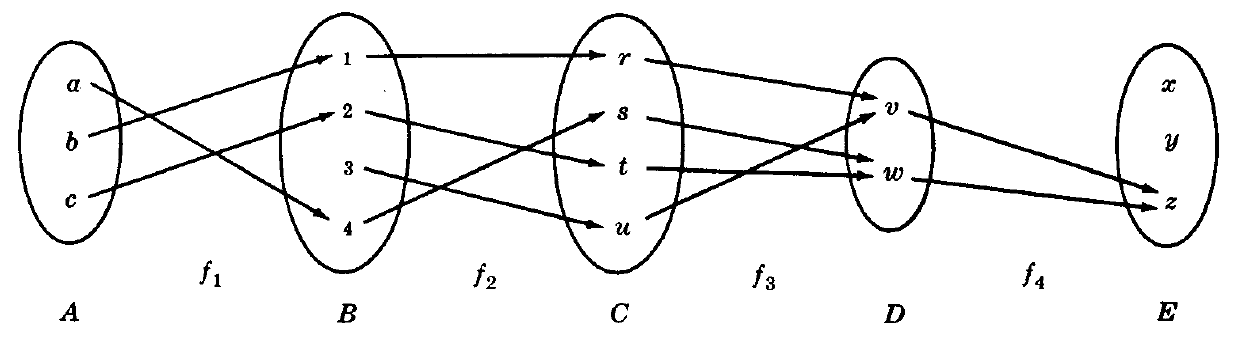
\includegraphics[width=10cm,keepaspectratio=true]{./md/MD02_IM01.png}
			% MD02_IM01.png: 0x0 pixel, 300dpi, 0.00x0.00 cm, bb=
			\label{fig:MD0201}
		\end{figure}
		
	\end{problema}
	



\subsection{Como encontrar funciones inversas}


Si $f:A \to B$ no es \emph{sobre,} es decir, $f(A) \subset B$ pero $f(A)\neq B,$ basta restringir su codominio a la imagen $f(A)$ para que se convierta en {sobre}:
$$
f: A \to f(A).
$$



\begin{problema}
La función $f:\R \to \R, x \mapsto x^{2}$ no es sobre, pero como 
$$f(A)=\set{x^2\mid x\in\R}=\set{y\in \R \mid y\geq 0}$$
la función $f: \R\to \set{y \geq 0}, x \mapsto x^{2}$ sí lo es.
\end{problema}




\begin{figure}[h!]
\centering
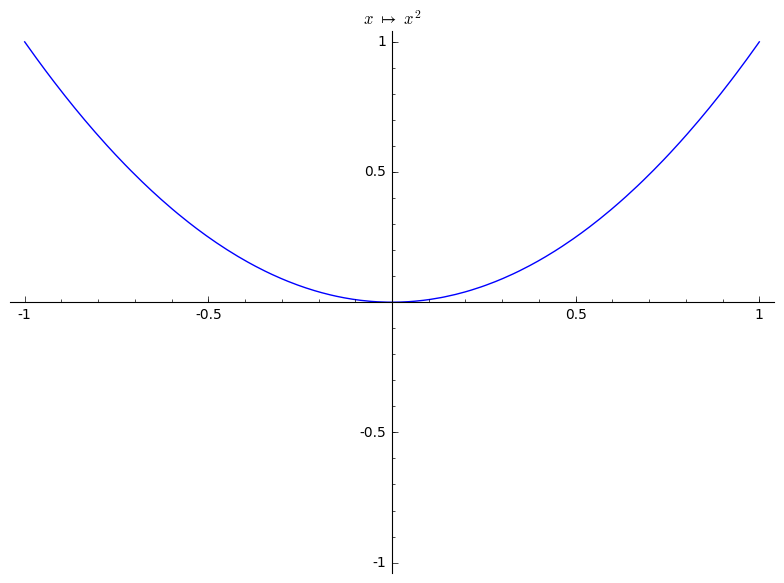
\includegraphics[width=8cm,keepaspectratio=true]{./md/IMG-04_resticcion.png}
% IMG-04_resticcion.png: 0x0 pixel, 300dpi, 0.00x0.00 cm, bb=
\caption{Gráfica de $x^2$}
\label{fig:0401}
\end{figure}




\begin{prop}
Si una función $f:A \to B$ es inyectiva, entonces
$$
f:A \to f(A)
$$ es invertible.
\end{prop}



{Como encontrar la inversa de $y=f(x)$}
\begin{enumerate}[(a)]
\item Verifique que $f(x)$ es un función $1:1.$ 
\item Despeje la variable independiente $y$ en la ecuación $y=f(x)$ para obtener
$$x=f^{-1}(y).$$ 
\item Reescriba la ecuación anterior intercambiando las variables: $y=f^{-1}(x).$
\end{enumerate}




\begin{problema}
Encuentre la inversa de la función $f(x)=3x-2,$
\end{problema}




\begin{problema}
Encuentre la inversa de $f(x)=\dfrac{x^{5}-3}{2}.$
\end{problema}




\begin{problema}
Encuentre la inversa de $f(x)=\sqrt{x-2}.$
\end{problema}




\begin{figure}[h!]
\centering
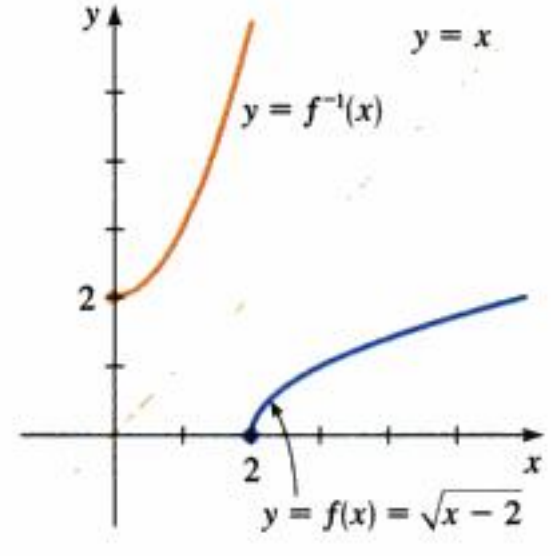
\includegraphics[height=8cm,keepaspectratio=true]{./md/MD02_sqrt_x-2.png}
% MD02_sqrt_x-2.png: 0x0 pixel, 300dpi, 0.00x0.00 cm, bb=
\label{fig:MD02_sqrt_x-2}
\end{figure}


%
\subsection{Caracterización geom\'etrica}


Consiere ahora una función $f:\R \to \R.$ Representemos su gráfica 
$$
\Gamma_{f}=\set{(x,y)\in\R^{2}\mid y=f(x)}
=\set{(x,f(x))}
$$
en el plano.




\begin{rem}
\begin{itemize}
\item $f:\R \to \R$ es \emph{$1:1$} si cada línea \emph{horizontal} intersecta la gráfica de $f$ a lo más en un punto.
\item $f:\R \to \R$ es \emph{sobre} si cada línea horizontal intersecta la gráfica de $f$ al menos en un punto.
\item $f:\R \to \R$ es \emph{invertible} si cada línea horizontal intersecta la gráfica de $f$...
\end{itemize}

\end{rem}



\begin{problema}
Considere las siguientes funciones $:\R \to \R$
\begin{enumerate}
\item $x \mapsto x^{2}$
\item $x \mapsto 2^{x}$
\item $x \mapsto x^{3}-2x^{2}-5x+6$
\item $x \mapsto x^{3}$
\end{enumerate}
y determine si son $1:1,$ sobre o invertibles.
\end{problema}




\begin{figure}[h!]
\centering
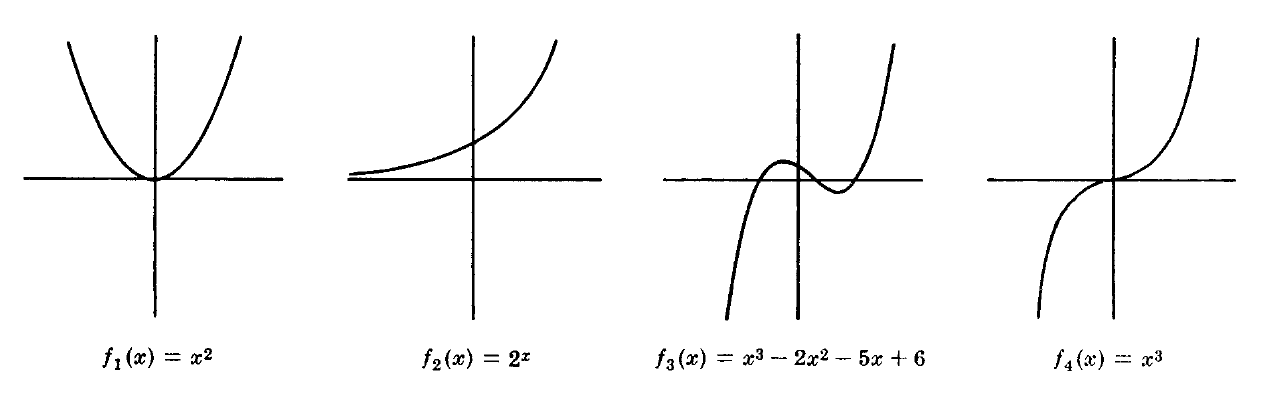
\includegraphics[width=10cm]{./md/MD02_IM02.png}
% MD02_IM02.png: 0x0 pixel, 300dpi, 0.00x0.00 cm, bb=
\label{fig:MD0202}
\end{figure}



\subsection{Permutaciones}


Consideremos un conjunto finito $X=\set{x_{1},...,x_{N}},$ esto es, $X$ tiene \emph{cardinalidad} $n(X)=N < \infty.$


Una función biyectiva (invertible) $\sigma:X \to X$ es llamada \emph{permutación} en $X.$


Observe que las composiciones e inversas de permutaciones, así como la identidad, son tambi\'en permutaciones.


En este caso, diremos que la permutación $\sigma$ \emph{actua} en $X.$



Supongamos que la permutación $\sigma$ actua en $X={x_{1},x_{2},x_{3}}$ de la siguiente manera:
$$
\sigma(x_{1})=x_{2}, \; \sigma(x_{2})=x_{3}, \; \sigma(x_{3})=x_{1}.
$$

Entonces, podemos representar la permitación de la siguiente manera
$$\sigma=
\begin{pmatrix}
1 & 2 & 3 \\
2 & 3 & 1,
\end{pmatrix},
$$  es decir, sólo nos fijamos de que manera actua en el índice $j$ del elemento $x_{j}.$



De manera general, numerando los elemenos de $X=\set{x_{1},...,x_{N}},$ podemos identificar este conjunto con $A_{N}=\set{1,...,N}$ por medio de la biyección $x_{i} \mapsto i.$


Ahora, consideremos una permutación $\sigma:A_{N}\to A_{N},$ tal que $\sigma(i)=\sigma_{i}.$ Entonces podemos representa $\sigma$ por medio de 
$$\sigma=
\begin{pmatrix}
1& ... & N \\
\sigma_{1}& ... & \sigma_{N}.
\end{pmatrix}
$$


El conjunto de todas las permutaciones $:A_{N}\to A_{N}$ se denota por $S_{N}$ y tiene una cardinalidad 
$n(S_{N})=N!.$



\chapter{Teoría de gráficos}
\section{Matrices}


Las matrices son arreglos rectangulares de número que nos ayudan a codificar información. Por ejemplo:
$$
\begin{pmatrix}
	a_{1,1} & a_{1,2} \\
	a_{2,1} & a_{2,2}
\end{pmatrix}
$$
puede ser útil para codificar los coeficientes del sistema de ecuaciones:
$$
\begin{cases}
	a_{1,1}x+a_{1,2}y=b_{1}\\
	a_{2,1}x+a_{2,2}y=b_{2}
\end{cases}
$$



En general, una matriz tiene la forma 
\begin{equation}
	\label{A}
	\tag{A}
	\begin{pmatrix}
		a_{1,1} & a_{1,2} & \cdots & a_{1,n} \\
		\vdots & & & \vdots\\
		a_{m,1} & a_{m,2} & \cdots & a_{m,n} 
	\end{pmatrix}
\end{equation} 

Los subíndices de cada elemento $a_{i,j}$ denotan la posición del mismo: $i$ es el número del \emph{renglón} (contando de arriba a abajo), mientras que $j$ es el número de la columna (contanto de izquierda a derecha).



Podemos extraer renglones y columnas de la matrix \eqref{A}: El $i-$esímo renglón es
$$
R_{i}=
\begin{pmatrix}
	a_{i,1} & \cdots & a_{i,n}
\end{pmatrix}
$$ 
mientras que la $j-$\'esima columna será
$$
C_{j}=
\begin{pmatrix}
	a_{j,1} \\
	\vdots \\
	a_{j,m}
\end{pmatrix}
$$



Diremos que la matriz \eqref{A} tiene dimensión $m\times n.$ 

Si existe un conjunto de números $F,$ tal que todos los elementos $a_{i,j}$ de la matriz pertenecen a dicho conjunto, diremos que la matriz tiene coeficientes en $F.$ 



\begin{rem}
	Para que las operaciones entre matrices est\'en bien definidas, es necesario que la suma, resta y multiplicación entre entre elementos de $F$ tambi\'en este bien definida. Por esto generalmente $F$ se elige como $\R$ o $\Z.$ 
\end{rem}



La colección de todas las matrices de dimensión $m\times n$ con coeficientes en $F$ se denotará por $$M_{m,n}(F).$$



\begin{defn}
	Las matrices de dimensión $m\times 1$ se conocen como \emph{vectores columna,} mientras que las de dimensión $1\times n$ se conocen como \emph{vectores renglón.}
	
	
	La colección $M_{m,1}(F)$ de todos los vectores columna con coeficientes  comunmente se denota por $F^{m}.$  Mientras que la colección $M_{1,n}(F)$ de todos los vectores columna con coeficientes  comunmente se denota por $F^{n\ast}.$
	
\end{defn}


\subsection{Operaciones elementales}


Por brevedad, la matriz \eqref{A} se denota por $A=[a_{i,j}].$ 

En el caso de los vectores renglones y columnas, podemos omitir el subíndice fijo
$$R=[R_{1,j}]=[R_{j}], \; C=[C_{i,1}]=[C_{i}].$$



Si $B=[b_{i,j}]$ es otra matriz de dimensión $m\times n,$ la suma se define como $$A+B=[a_{i.j}+b_{i,j}].$$ 

De manera similar, la resta se define como $$A-B=[a_{i,j}-b_{i,j}].$$



\begin{problema}
	$$
	\begin{pmatrix}
		1 & -1 & 0 \\
		2 & 3 & -4
	\end{pmatrix}
	+
	\begin{pmatrix}
		7 & 0 & -1 \\
		2 & -1 & 5
	\end{pmatrix} =
	$$ 
	$$
	\begin{pmatrix}
		1 & -1 & 0 \\
		2 & 3 & -4
	\end{pmatrix}
	-
	\begin{pmatrix}
		7 & 0 & -1 \\
		2 & -1 & 5
	\end{pmatrix} =
	$$
\end{problema}




Observe que para que la \emph{suma y resta} tenga sentido, ambas matrices deben tener exactamente las \emph{mismas dimensiones}. 

Despu\'es de ver la facilidad para definir la suma y resta, uno se ve tentado a definir la multiplicación de la misma forma. Pero tal definición es poco útil en las aplicaciones. 

Por esta razón, desarrollaremos el concepto de multiplicación, a fin de poder aplicar esta operación en la resolución de Ejemplos.


\subsection{Multiplicación}

\begin{defn}
	Sean $R=[R_{j}]$ un vector renglón y $C=[C_{i}]$ un vector columna, ambos de longitud $n.$
	
	El \emph{producto renglón-columna} se define como
	\begin{equation}
		\label{RC}
		\tag{RC}
		RC=
		\begin{pmatrix}
			R_{1}& \cdots & R_{n}
		\end{pmatrix}
		\begin{pmatrix}
			C_{1} \\ \vdots \\ C_{n}
		\end{pmatrix}
		=
		\sum_{i=1}^{n} R_{j}C_{i}.
	\end{equation}
	
\end{defn}




\begin{problema}
	Considere
	$$
	R=
	\begin{pmatrix}
		1 & 0 & -1
	\end{pmatrix}, \;
	C=
	\begin{pmatrix}
		2\\ 1 \\ -2
	\end{pmatrix}.
	$$
	
	Calcule $RC.$
	
\end{problema}




\begin{problema}
	Reescriba la siguiente ecuación, utilizando el \emph{producto renglón-columna}:
	$$2x-3y+z=0.$$
\end{problema}




\begin{defn}
	Sea $A=[a_{i,j}]\in M_{m\times n}$ y $B=[b_{j,k}]\in M_{n\times l}.$ Definimos su producto como
	\begin{equation}
		\label{AB}
		\tag{AB}
		AB=
		\begin{pmatrix}
			R_{i}C_{k}
		\end{pmatrix}
	\end{equation}
	donde $R_{i}$ es el $i-$\'esimo renglón de $A$ y $C_{k}$ es la $k-$\'esima columna de $B.$
\end{defn}




\begin{rem}
	\begin{itemize}
		\item Para que esta multiplicación tenga sentido, los renglones de $A$ y las columnas de $B$ deberán tener la misma longitud $n.$
		
		\item La matriz resultante tendrá dimensión $m \times l.$  
		\item A menos que $m=l,$ el producto $BA$ podría no estar definido. 
		\item Aun cuando $BA$ estuviera bien definido, el producto de matrices no es \emph{conmutativo,} es decir, generalmente tendremos que $$AB \neq BA.$$
	\end{itemize}
\end{rem}




\begin{problema}
	Encuentre el producto $AB$ de las siguientes matrices
	$$A= \left(\begin{array}{r}
		0
	\end{array}\right) $$
	$$B= \left(\begin{array}{rr}
		0 & -1
	\end{array}\right) $$
	Solución:
	$$AB= \left(\begin{array}{rr}
		0 & 0
	\end{array}\right) $$
\end{problema}



\begin{problema}
	Encuentre el producto $AB$ de las siguientes matrices
	$$A= \left(\begin{array}{rr}
		0 & -1 \\
		-1 & 0 \\
		0 & 0
	\end{array}\right) $$
	$$B= \left(\begin{array}{rrr}
		0 & -1 & 0 \\
		0 & 0 & 0
	\end{array}\right) $$
	Solución:
	$$AB= \left(\begin{array}{rrr}
		0 & 0 & 0 \\
		0 & 1 & 0 \\
		0 & 0 & 0
	\end{array}\right) $$
\end{problema}



\begin{problema}
	Encuentre el producto $AB$ de las siguientes matrices
	$$A= \left(\begin{array}{r}
		-1 \\
		-1 \\
		0
	\end{array}\right) $$
	$$B= \left(\begin{array}{rrr}
		-1 & 0 & 0
	\end{array}\right) $$
	Solución:
	$$AB= \left(\begin{array}{rrr}
		1 & 0 & 0 \\
		1 & 0 & 0 \\
		0 & 0 & 0
	\end{array}\right) $$
\end{problema}



\begin{problema}
	Encuentre el producto $AB$ de las siguientes matrices
	$$A= \left(\begin{array}{r}
		6 \\
		-9 \\
		-10
	\end{array}\right) $$
	$$B= \left(\begin{array}{r}
		-5
	\end{array}\right) $$
	Solución:
	$$AB= \left(\begin{array}{r}
		-30 \\
		45 \\
		50
	\end{array}\right) $$
\end{problema}



\begin{problema}
	Encuentre el producto $AB$ de las siguientes matrices
	$$A= \left(\begin{array}{r}
		2
	\end{array}\right) $$
	$$B= \left(\begin{array}{rrr}
		-1 & 1 & -3
	\end{array}\right) $$
	Solución:
	$$AB= \left(\begin{array}{rrr}
		-2 & 2 & -6
	\end{array}\right) $$
\end{problema}



\begin{problema}
	Encuentre el producto $AB$ de las siguientes matrices
	$$A= \left(\begin{array}{rr}
		-1 & -3 \\
		-7 & -1
	\end{array}\right) $$
	$$B= \left(\begin{array}{r}
		-7 \\
		-4
	\end{array}\right) $$
	Solución:
	$$AB= \left(\begin{array}{r}
		19 \\
		53
	\end{array}\right) $$
\end{problema}



\begin{problema}
	Rescriba el siguiente sistema de ecuación en forma matricial y encuentre su solución:
	$$
	\begin{cases}
		-x-3y=19\\
		-7x-y=53
	\end{cases}
	$$
\end{problema}




\section{Teoría general de grafos}


	En matemáticas, la \emph{teoría de grafos} estudia estructuras matemáticas usadas para modelar relaciones por pares entre objetos. 


\subsection{Definición de grafo}

{Concepto de gráfo}
	Un \emph{grafo} $G$ consiste de:
	\begin{enumerate}[(a)]
		\item Un conjunto $V$ cuyos elementos son llamados \emph{v\'ertices,} puntos o nodos de $G.$
		\item Un conjunto $E$ de pares (no ordenados) de distintos vertices, a los que llamaremos \emph{aristas} de $G.$
	\end{enumerate}
	
	Denotaremos un grafo por $G(V,E)$ cuando querramos enfatizar los componentes del mismo.



	\begin{rem}
		Debido a una ambig\"uedad en la traducción del ingl\'es al espa\~nol, en ocasiones, a un grafo tambi\'en se le conoce como \emph{gráfica,} que se puede confundir con el concepto de teoría de conjuntos. En este material, a veces utilizaremos \textit{gráfica,} pero debe entenderse como un grafo. 
	\end{rem}



	\begin{figure}[h!]
		\centering
		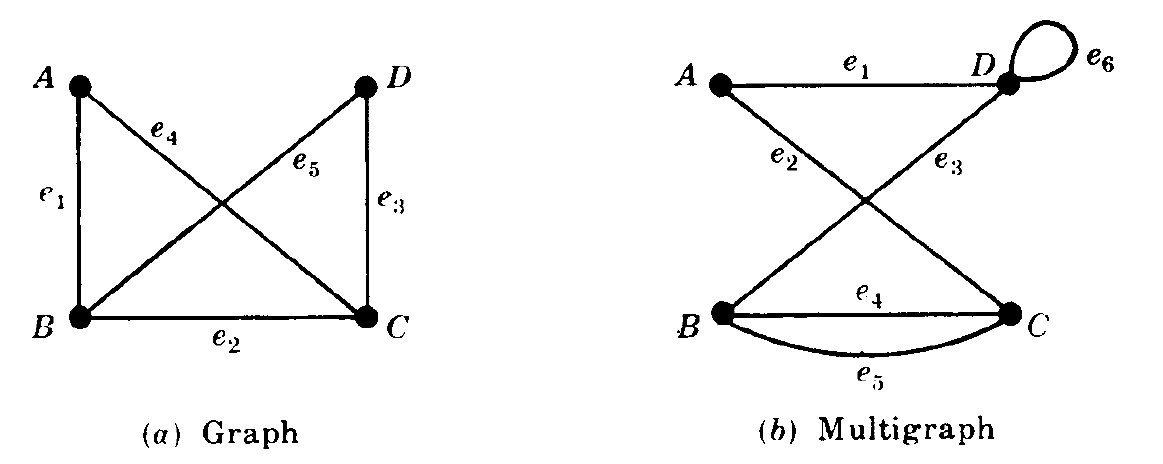
\includegraphics[width=12cm,keepaspectratio=true]{./md/grafos.png}
		% grafos.png: 0x0 pixel, 300dpi, 0.00x0.00 cm, bb=
		\caption{Grafos y multigrafos}
		\label{fig:md0501}
	\end{figure}
	


{Multigrafos}
	Consideremos la figura \ref{fig:md0501} (b). Las aristas $e_{4}$y $e_{5}$ son llamadas \emph{aristas multiples} ya que conectan los mismos extremos,  mientras que la arista $e_{6}$ es llamada \emph{bucle} ya que conecta un v\'ertice consigo mismo. 
	



	Tales diagramas son llamados \emph{multigrafos;}  la definición formal de grafo no admite aristas multiples ni bucles. 



	\begin{rem}
		Sin embargo, algunos textos utilizan ``grafos'' para referirse a lo que nosotros llamaremos multigrafos, mientras que ocupan ``grafo simple'' para lo que nosotros llamaremos grafos.
	\end{rem}
	


{Grado de un v\'ertice}
	El \emph{grado} de un v\'ertice $v$ es un grafo $G,$ denotado por $\deg(v),$ es igual al número de aristas in $G$ que contienen a $v,$ es decir, que \emph{inciden} en $v.$



	Dado que cada arista incide en dos v\'ertices diferentes, tenemos el siguiente resultado simple pero importante:
	\begin{thm}
		La suma de los grados de los v\'ertices en un grafo $G$ es el doble del número de aristas. 
	\end{thm}
	



	\begin{problema}
		En el grafo de la figura \ref{fig:md0501}(a), tenemos que 
		$$\deg(A)=2, \; \deg(B)=3,\; \deg(C)=3, \; \deg(D)=2.$$
		
		
		La suma de los grados es igual a 10, que es dos veces el número de aristas. 
	\end{problema}
	



	\begin{defn}
		Diremos que un v\'ertice es \emph{par} o \emph{impar} de acuerdo a la paridad de su grado. 
		
		En el ejemplo anterior, tanto $A$ com $D$ son v\'ertices pares, mientras que $B$ y $C$ son impares.
	\end{defn}
	



	\begin{rem}
		Diremos que un vertice de grado cero está \emph{aislado.}
	\end{rem}


{Gráfos finitos y triviales}
	Diremos que un grafo  es \emph{finito} si tiene un número finito de v\'ertices y un número finito de aristas. 
	
	Observe que un número finito de v\'ertices implica un número finito de aristas; pero no lo contrario no es necesariamente cierto. 
	
	Diremos que un grafo con un único v\'ertice, sin aristas,  es \emph{trivial.}\



	\begin{rem}
		A menos que se indique de otra manera, sólo trataremos con grafos finitos. 
	\end{rem}
	


\subsection{Subgrafos y grafos homeomorfos e isomorfos}


	Ahora, discutiremos relaciones de equivalencia entre grafos.


{Subgrafos}
	Consideremos un grafo $G(V,E).$ Diremos que otro grafo $H(V',E')$ es un \emph{subgrafo} de $G$ si los v\'ertices y aristas de $H$ están contenidos en los v\'ertices y aristas de $G,$ es decir, 
	$$
	V'\subset V, \; E' \subset E.
	$$



	En particular:
	\begin{enumerate}[(a)]
		\item Un subgrafo $H(V',E')$ de $G(V,E)$ es llamado subgrafo \emph{inducido} por sus v\'ertices $V'$ si el conjunto de aristas $E'$ contiene todas las aristas en $G$ cuyo extremos pertenecen a los v\'ertices en $H.$ 
		\item Si $v$ es un v\'ertice en $G,$ entonces \emph{$G-v$} es el subgrafo de $G$ ontenido al borrar $v$ de $G$ y todas las aristas en $G$ que inciden en $v.$ 
		\item Si $e$ es una arista en $G,$ entonces \emph{$G-e$} es el subgrafo de $G$ obtenido borrando la arista $e$ en $G.$
	\end{enumerate}
	


{Grafos isomorfos}
	Dos grafos $G(V,E)$ y $G^{*}(V^{*},E^{*})$ son llamados \emph{isomorfos} si existe una función biyectiva $f: V \to V^{*}$ tal que: $\set{u,v}$ es una arista de $G$ si y solo si $\set{f(u),f(v)}$ es una arista de $G^{*}.$
	 
	
	La idea es que estos grafos son equivalentes, aún cuando sus representaciones pueden lucir muy diferentes.



	\begin{figure}[h!]
		\centering
		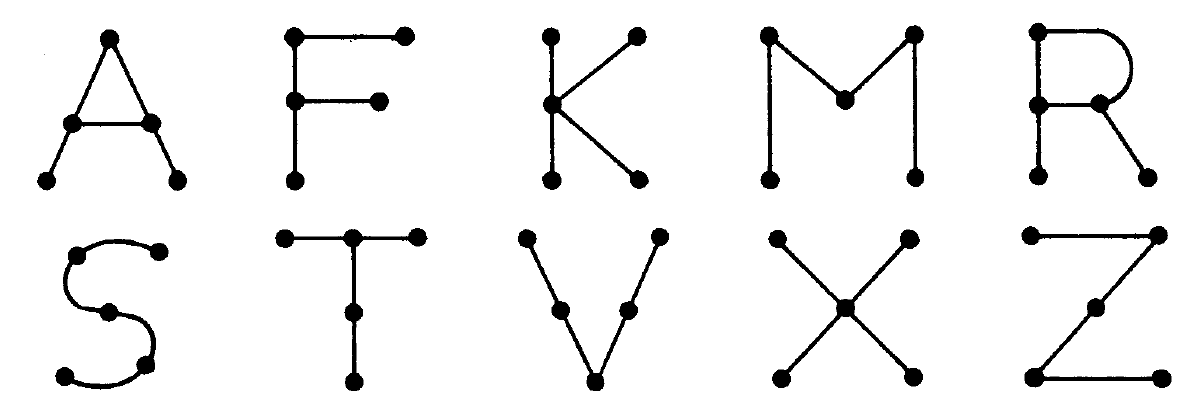
\includegraphics[width=10cm,keepaspectratio=true]{./md/letras.png}
		% letras.png: 0x0 pixel, 300dpi, 0.00x0.00 cm, bb=
		\caption{Grafos isomorfos.}
		\label{fig:md0502}
	\end{figure}
	


{Grafos homeomorfos}
	Dado un grafo $G,$ podemos obtener un nuevo grafo dividiendo una arista de $G$ con v\'ertices adicionales. 
	
	Dos grafos $G$ y $G^{*}$ son llamados \emph{homeomorfos} si pueden obtenerse de gráficas isomorfas a trav\'es de este m\'etodo. 



	\begin{figure}[h!]
		\centering
		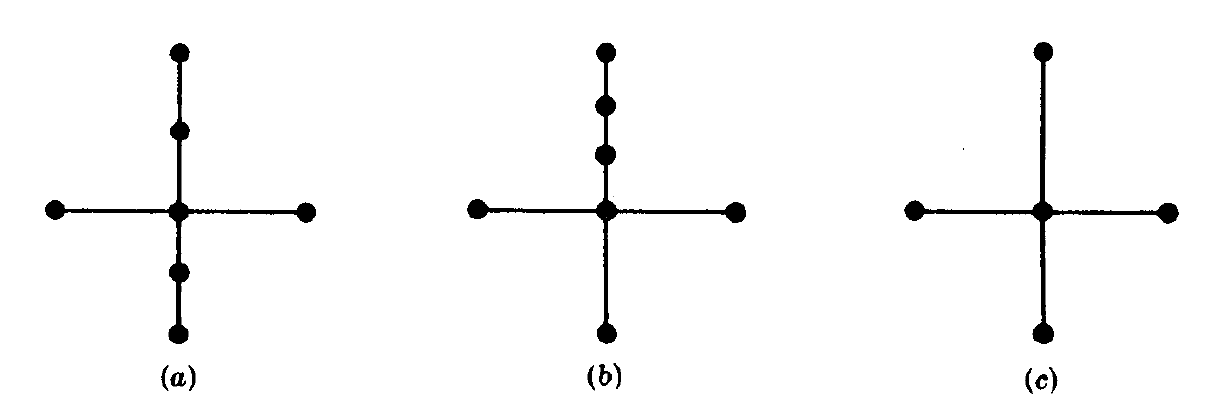
\includegraphics[width=8cm,keepaspectratio=true]{./md/homomorfas.png}
		% homomorfas.png: 0x0 pixel, 300dpi, 0.00x0.00 cm, bb=
		\caption{Grafos homomorfos}
		\label{fig:md0503}
	\end{figure}
	
	Los grafos $(a)$ y $(b)$ son homeomorfos, ya que se pueden obtener a\~nadiendo v\'ertices al grafo $(c).$


\subsection{Caminos y conexidad}


	Un \emph{camino} en un (multi)grafo $G$ consiste en una sucesión alternante de v\'ertices y arista de la forma
	$$
	v_{0}, e_{1}, v_{1}, ..., e_{n-1}, v_{n-1}, e_{n}, v_{n}
	$$
	donde cada arista $e_{i}$ contiene los v\'ertices $v_{i-1}$ y $v_{i}.$



	\begin{rem}
		Observe que en grafo, podemos simplificar la notación para un camino, indicando sólo los v\'ertices que recorre:
		$$v_{0}, v_{1},..., v_{n}.$$ 
	\end{rem}



	Diremos que el camino es \emph{cerrado} si $v_{n}=v_{0}.$ En otro caso, diremos que el camino conecta $v_{0}$ con $v_{n}.$
	 
	
	Un \emph{camino simple} es aquel en el cual todos los v\'ertices son distintos. Mientras que un camino en el que todas las aristas son distintas se llama \emph{paseo}.
	



	La \emph{longitud} de un camino es igual a número de aristas en la sucesión que lo define.
	 



	Un \emph{ciclo} es un camino cerrado de \emph{longitud} al menos 3, en el que todos los v\'ertices son distintos, excepto el inicial $v_{0}$ y el final $v_{n}.$
	
	
	Un ciclo de longitud $k$ es llamado \emph{$k-$ciclo.}



	\begin{figure}[h!]
		\centering
		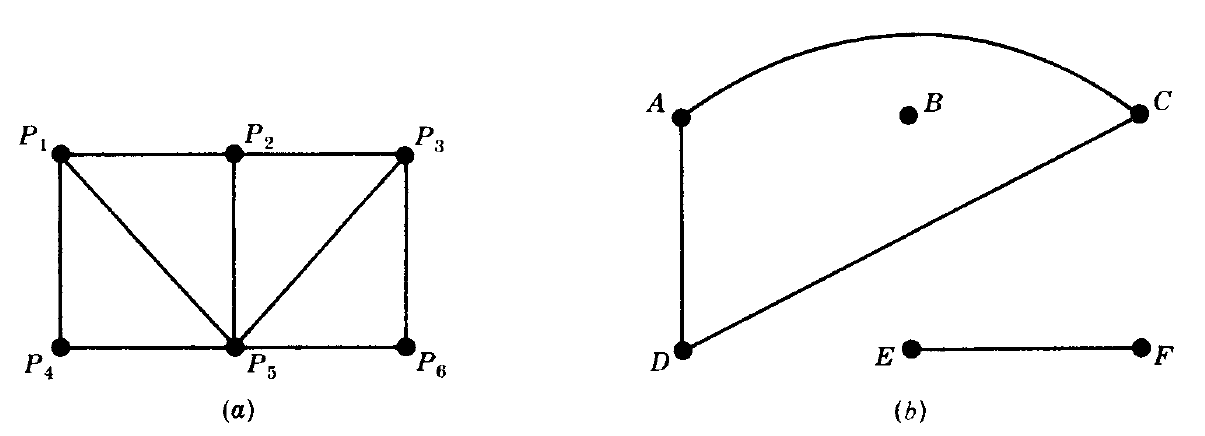
\includegraphics[width=10 cm,keepaspectratio=true]{./md/grafo_8_8.png}
		% grafo_8.8.png: 0x0 pixel, 300dpi, 0.00x0.00 cm, bb=
		\caption{Conexidad en grafos}
		\label{fig:md0504}
	\end{figure}



	\begin{problema}
		\label{lip:exmp:8.1}
		Consideremos el grafo \ref{fig:md0504}(a). Considere las siguientes sucesiones
		\begin{align*}
			\a&=\left( P_{4}, P_{1}, P_{2}, P_{5}, P_{1},P_{2}, P_{3}, P_{6}  \right), \\
			\b&=\left( P_{4}, P_{1}, P_{5}, P_{2}, P_{6} \right) \\
			\gam&= \left( P_{4}, P_{1}, P_{5}, P_{2}, P_{3}, P_{5}, P_{6} \right)\\
			\del&=\left( P_{4}, P_{1}, P_{5}, P_{3}, P_{6} \right).
		\end{align*}
		
	\end{problema}
	



	\begin{figure}[h!]
		\centering
		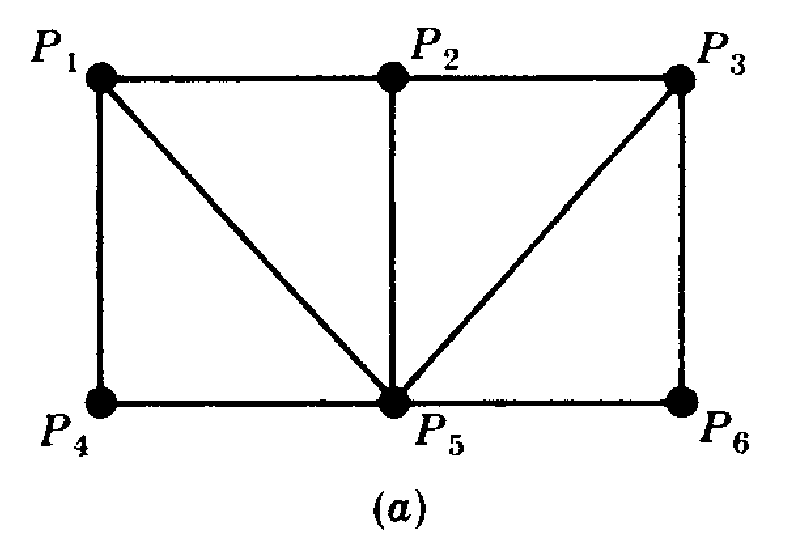
\includegraphics[width=5cm,keepaspectratio=true]{./md/grafo_8_8_a.png}
		% grafo_8_8_a.png: 0x0 pixel, 300dpi, 0.00x0.00 cm, bb=
	\end{figure}
	$\a$ es un camino de $P_{4}$ a $P_{6},$ pero no es un paseo.



	\begin{figure}[h!]
		\centering
		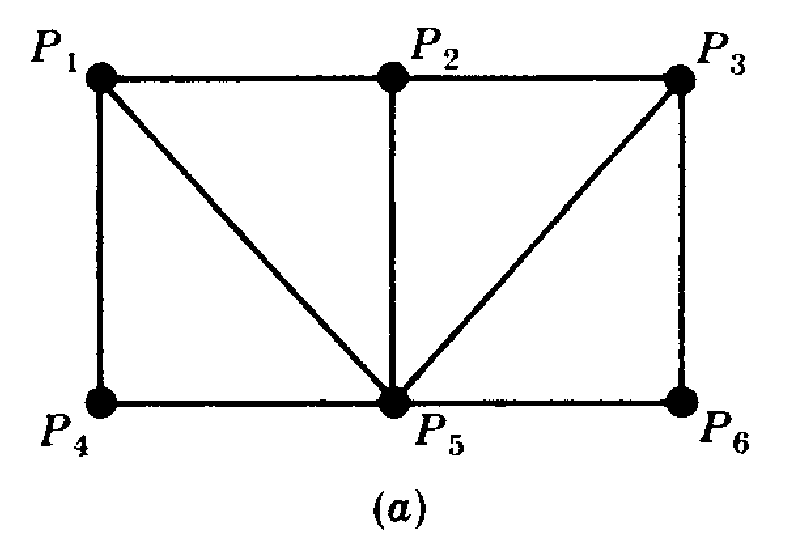
\includegraphics[width=5cm,keepaspectratio=true]{./md/grafo_8_8_a.png}
		% grafo_8_8_a.png: 0x0 pixel, 300dpi, 0.00x0.00 cm, bb=
	\end{figure}
	$\b$ no es un camino, ya que no existe alguna arista $\set{P_{2}, P_{6}}.$



	\begin{figure}[h!]
		\centering
		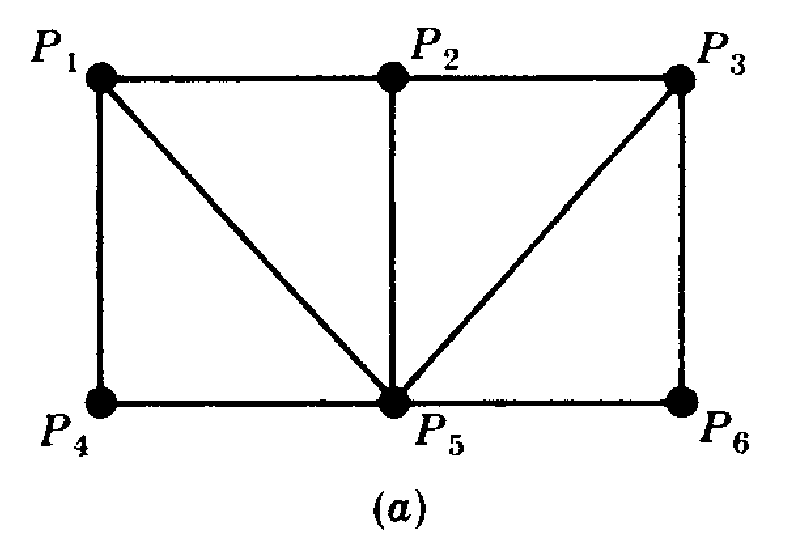
\includegraphics[width=5cm,keepaspectratio=true]{./md/grafo_8_8_a.png}
		% grafo_8_8_a.png: 0x0 pixel, 300dpi, 0.00x0.00 cm, bb=
	\end{figure}
	$\gam$ es un paseo, pero no es un camino simple.



	\begin{figure}[h!]
		\centering
		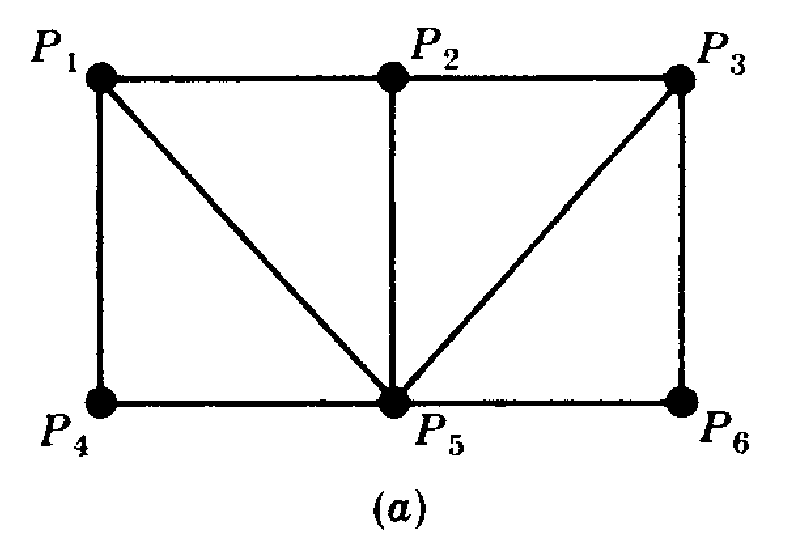
\includegraphics[width=5cm,keepaspectratio=true]{./md/grafo_8_8_a.png}
		% grafo_8_8_a.png: 0x0 pixel, 300dpi, 0.00x0.00 cm, bb=
	\end{figure}
	$\del$ es un camino simple de $P_{4}$ a $P_{6},$ pero no es el camino más corto, es decir, con el meno número de aristas. ?`Cuál es el camino más corto?



	Eliminando aristas innecesarias, no es difícil ver que cualquier camino de $u$ a $v$ puede ser reemplazado por un camino simple.
	 
	
	Formalmente:
	\begin{thm}
		Existe un camino del v\'ertice $u$ a $v$ si y solo si existe un camino simple de $u$ a $v.$
	\end{thm}
	


{Conexidad y componentes conexas}
	Un grafo $G$ es conexo si existe un camino entre cualesquiera dos v\'ertices.  Por ejemplo, el grafo \ref{fig:md0504}(a) es conexo, pero no así el grafo \ref{fig:md0504}(b).
	\begin{figure}[h!]
		\centering
		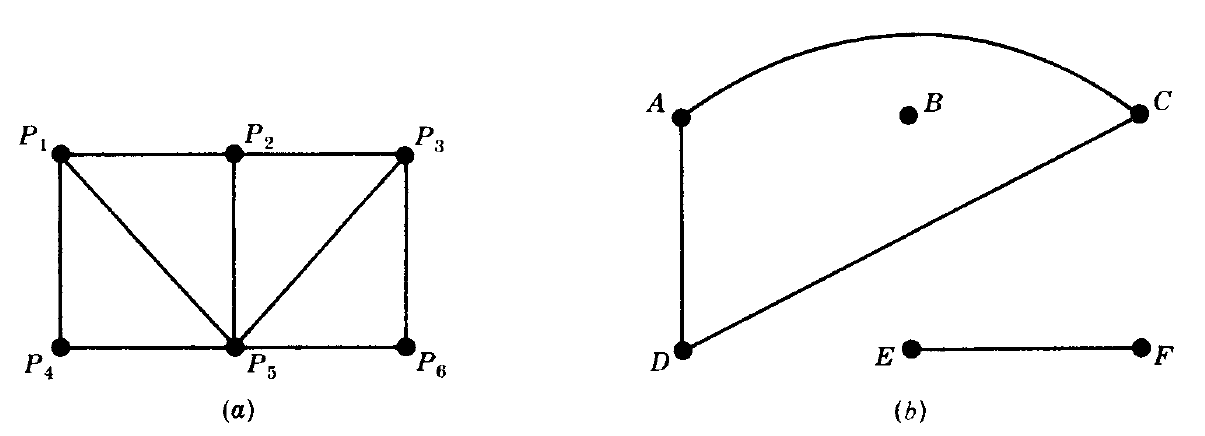
\includegraphics[width=8cm,keepaspectratio=true]{./md/grafo_8_8.png}
		% grafo_8_8.png: 0x0 pixel, 300dpi, 0.00x0.00 cm, bb=
	\end{figure}
	



	Consideremos un grafo $G.$ Un subgrafo conexo $H$ de $G$ es llamado \emph{componente conexa} de $G$ si $H$ no está contenido de manera propia en cualquier otro grafo conexo de $G.$ 
	
	Por ejemplo, el grafo \ref{fig:md0504}(b) tiene tres componentes conexas.
	
	\begin{figure}[h!]
		\centering
		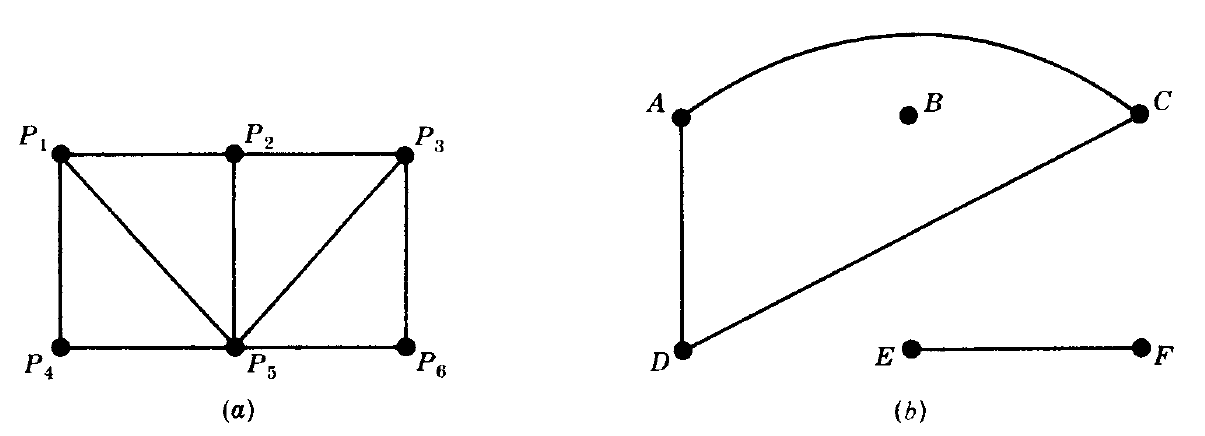
\includegraphics[width=8cm,keepaspectratio=true]{./md/grafo_8_8.png}
		% grafo_8_8_a.png: 0x0 pixel, 300dpi, 0.00x0.00 cm, bb=
	\end{figure}
	



	\begin{rem}
		Formalmente, permitiendo que un v\'ertice $u$ est\'e conectado consigo mismo, la relación \begin{center}
			\texttt{$u$ está conectado con $v$}                                                                                                                                                                                            \end{center}
		es una relación de equivalencia en el conjunto de v\'ertices del grafo $G,$  y las clases de equivalencia de esta relación son las componentes conexas de $G.$
	\end{rem}
	


{Distancia y diametro}
	Consideremos un grafo conexo $G.$ La distancia entre  dos v\'ertices $u$ y $v$ en $G,$ denotada por $d(u,v),$ es la longitud del camino más corto entre $u$ y $v.$ E\~n diametro de $G,$ escrito $diam(G),$ es la distancia máxima entre cualesquiera dos puntos en $G.$ 



	\begin{figure}[h!]
		\centering
		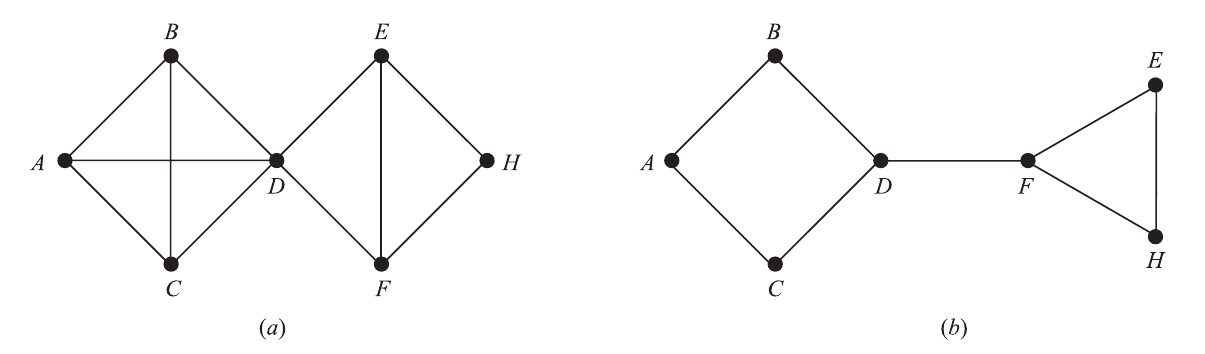
\includegraphics[width=10cm,keepaspectratio=true]{./md/grafo_8_9.png}
		% grafo_8_9.png: 0x0 pixel, 300dpi, 0.00x0.00 cm, bb=
		\caption{Distancia y diametro}
		\label{fig:md0505}
	\end{figure}
	Por ejemplo, en el grafo \ref{fig:md0505}(a), el diamtero es $3,$ mientras que en el (b), el diametro es 4.


{Puntos de corte y puentes}
	Sea $G$ un grafo conexo. Un v\'ertice $v$ en $G$ es llamado \emph{punto de corte} si $G-v$ es disconexo. Una arista $e$ en $G$ es llamada \emph{puente} si $G-e$ es disconexo. 
	
	\begin{figure}[h]
		\centering
		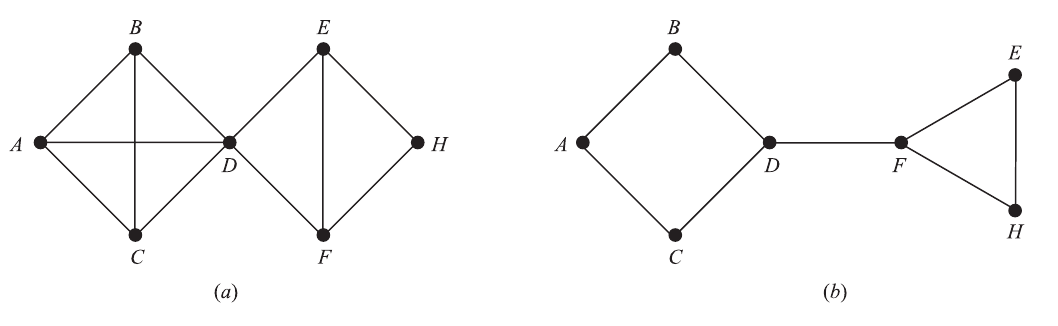
\includegraphics[height=3cm,keepaspectratio=true]{./md/fig0809.png}
		% fig0809.png: 0x0 pixel, 300dpi, 0.00x0.00 cm, bb=
		\caption{Puntos de corte y puentes}
		\label{fig:0809}
	\end{figure}
	


\subsection{Grafos transitables y eulerianos}

	\begin{figure}[h!]
		\centering
		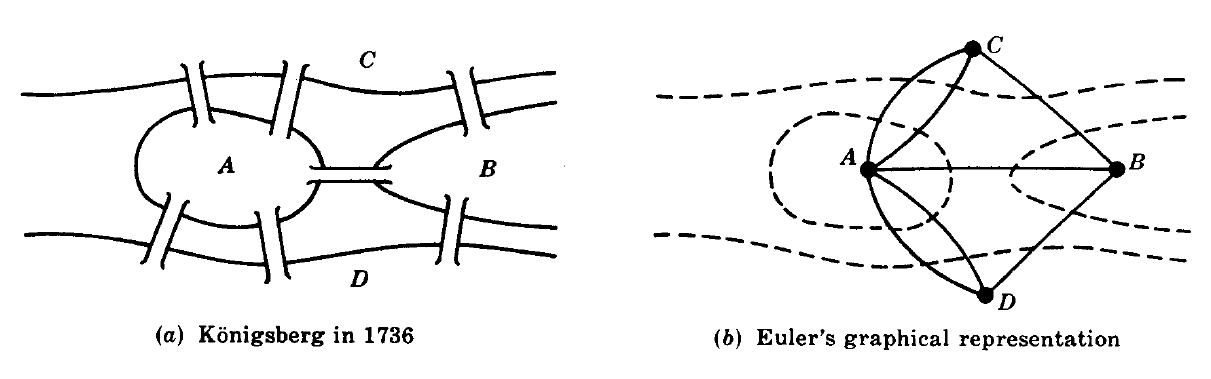
\includegraphics[width=10cm,keepaspectratio=true]{./md/grafo_8_10.png}
		% grafo_8_10.png: 0x0 pixel, 300dpi, 0.00x0.00 cm, bb=
		\caption{Puentes de K\"onigsberg y su representación}
		\label{fig:md0506}
	\end{figure}



	Un multigrafo es llamado \emph{transitable} si existe un \emph{paseo} (un camino dónde todos las aristas son diferentes), que incluye \emph{todos los v\'ertices y todas las aristas.}
	
	Tal paseo será llamado  \emph{paseo transitable}. 
	
	
	\begin{rem}
		De manera equivalente, un paseo transitable es un camino en el que todos los v\'ertices se transitan \emph{al menos} una vez,  pero las aristas \emph{exactamente} una vez.
	\end{rem}
	



	
	\begin{prop}
		Cualquier grafo conexo y finito con exactamente dos v\'ertices impares es transitable. Un paseo transitable puede comenzar en alguno de los v\'ertices impares y terminar en el otro v\'ertice impar.
	\end{prop}



	Un grafo $G$ es llamado \emph{grafo Euleriano} si existe un \emph{paseo transitable cerrado}.
	
	
	A tal paseo le llamaremos \emph{paseo Euleriano.}
	
	
	\begin{thm}[Euler]
		Un grafo conexo y finito es Euleriano si y solo si cada v\'ertice tiene grado par. 
	\end{thm}
	


{Grafos hamiltonianos}
	En la definición de grafos Eulerianos se enfatizó pasar por todas las aristas. 
	
	
	Ahora, nos enfocaremos en visitar todos los v\'ertices. 



	Un \emph{circuito Hamiltoniano} es un grafo $G$ es un camino cerrado que visita cada v\'ertice en $G$ \emph{exactamente} una vez.
	
	
	Si $G$ admite un circuito Hamiltoniano, entonces $G$ es llamado un \emph{grafo Hamiltoniano.}
	
	
	\begin{rem}
		En la definición de circuito Hamiltoniano, cuando decimos que el camino \emph{visita} cada v\'ertice exactamente una vez significa que, aunque el v\'ertice inicial tiene que ser el mismo que el final, todos los demás v\'ertices intermedios deben ser distintos.
	\end{rem}
	



	\begin{rem}
		Un {\color{red}paseo Euleriano} atraviesa {\color{red}cada una de las aristas} exactamente una vez, pero los v\'ertices se pueden repetir, mientras que un {\color{blue}circuito Hamiltoniano} visita {\color{blue}cada uno de los v\'ertices} exactamente una vez, pero las aristas pueden repetirse. 
		
		
	\end{rem}
	
	
	
	\begin{thm}
		Sea $G$ un grafo conexo con $n$ v\'ertices. Entonces $G$ es Hamiltoniano si $n\geq 3$ y $n \leq \deg(v)$ para cada v\'ertice $v$ en $G.$
	\end{thm}
	



	\begin{figure}[h!]
		\centering
		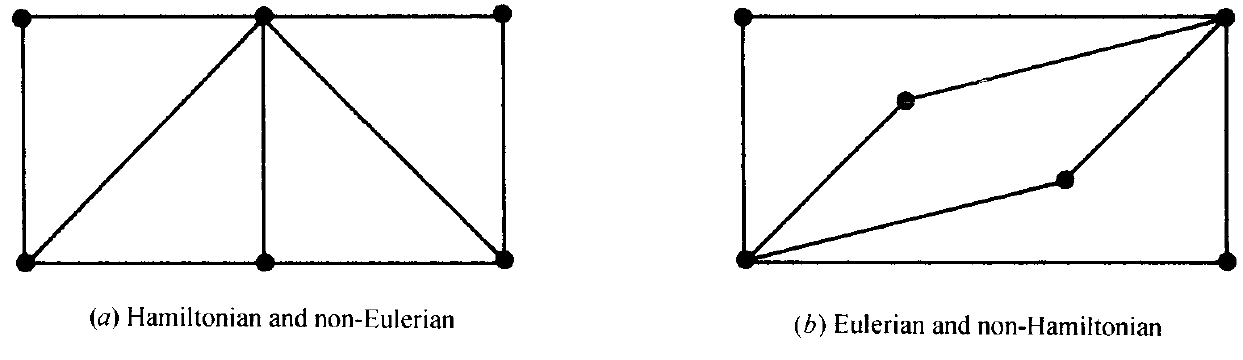
\includegraphics[width=10 cm]{./md/grafo_8_11.png}
		% grafo_8_11.png: 0x0 pixel, 300dpi, 0.00x0.00 cm, bb=
		\caption{Circuitos Eulerianos y Hamiltonianos}
		\label{fig:md 0506}
	\end{figure}
	



\subsection{Matriz de adyacencia}


	Supongamos que $G$ es un gráfo con $m$ v\'ertices y que estos han sido ordenados:
	$$
	v_{1}, v_{2},...,v_{m}.
	$$
	
	Entonces, la \emph{matriz de adyacencia} $A=\left( a_{i,j} \right)$ del grafo $G$ es la matriz de dimensión $m\times m$ definida por:
	$$a_{i,j}=
	\begin{cases}
		1 & v_{i}\texttt{ es adyacente a }v_{j}\\
		0 & \texttt{en otro caso}
	\end{cases}
	$$



	\begin{figure}[h]
		\centering
		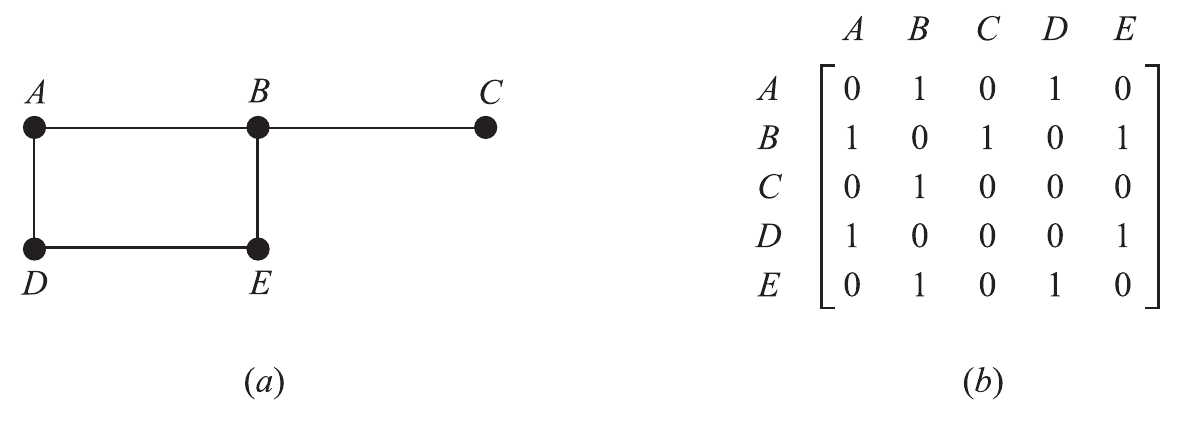
\includegraphics[width=10cm,keepaspectratio=true]{./md/fig0827.png}
		% fig0827.png: 0x0 pixel, 300dpi, 0.00x0.00 cm, bb=
		\caption{Matriz de adyacencia}
		\label{fig:0827}
	\end{figure}
	



\section{Digrafos}


Los \emph{grafos dirigidos} o \emph{digrafos} son grafos en los que las aristas tienen una direcci\'on.


\subsection{Grafos dirigidos}


Un grafo dirigido $G=G(V,E)$ consiste de:
\begin{enumerate}
	\item Un conjunto $V=V(G)$ cuyos elementos son llamados \emph{v\'ertices};
	\item un conjunto $E=E(G)$ de \emph{pares ordenados} ordenados de v\'ertices llamados \emph{arcos} o \emph{aristas dirigidas.}
\end{enumerate}




Supongamos que $e=(u,v)$ es un arco en el digrafo $G.$ Entonces, la siguiente terminolog\'ia es usada:
\begin{itemize}
	\item $e$ comienza en $v$ y termina en $v;$
	\item $u$ es el origen o punto inicial de $e,$ mientras que $v$ es el destino o punto final de $e.$
	\item $v$ es un sucesor de $u;$
	\item $u$ es adyacente a $v$ y $v$ es adyacente desde $u.$
\end{itemize}


Si $u=v,$ $e$ es llamado un \emph{bucle.}



Si las aristas o los v\'ertices de un digrafo est\'an etiquetas con alg\'un tipo de dato, diremos que es un \emph{digrafo etiquetado.}


De manera similar a un grafo, un digrafo ser\'a finito si el conjunto de v\'ertices y el de aristas es finito.



\begin{exmp}
	Consideremos el siguiente digrafo.
	\begin{figure}[h]
		\centering
		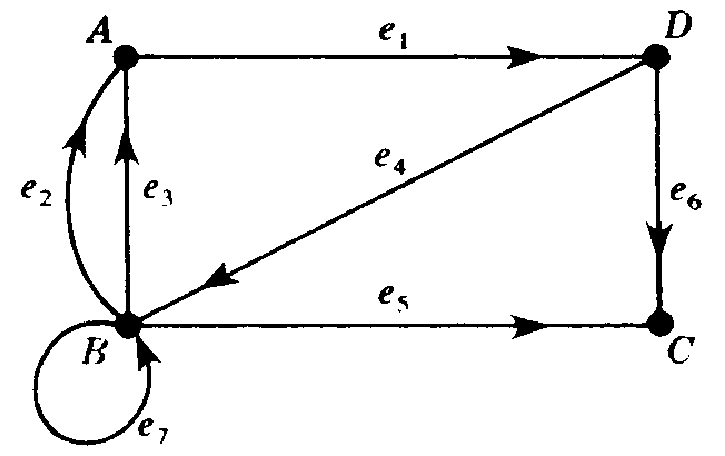
\includegraphics[height=3cm,keepaspectratio=true]{./md/fig0901a.png}
		% fig0901a.png: 0x0 pixel, 300dpi, 0.00x0.00 cm, bb=
		%\caption{Digrafo}
		\label{fig:0901a}
	\end{figure}
	Las aristas $e_{2}$ y $e_{3}$ son llamados \emph{paralelos,} ya que ambos comienzan en $B$ y terminan en $A.$ La arista $e_{7}$ es un \emph{bucle.}
\end{exmp}




\begin{exmp}
	\begin{figure}[h]
		\centering
		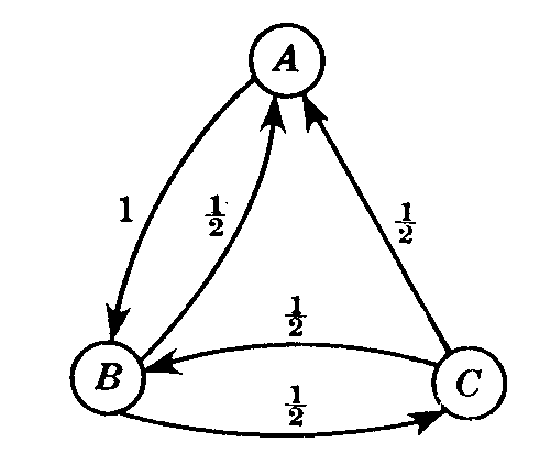
\includegraphics[width=5cm,keepaspectratio=true]{./md/fig0901b.png}
		% fig0901b.png: 0x0 pixel, 300dpi, 0.00x0.00 cm, bb=
		\caption{Proceso estocástico}
		\label{fig:0901b}
	\end{figure}
	
\end{exmp}



\subsection{Matriz de adyacencia}


Ahora, s\'olo consideraremos \emph{digrafos simples} $G(V,E)$, es decir, sin aristas paralelas. Entonces $E$ es simplemente una relaci\'on en $V.$ 

De manera inversa, si $R$ es una relaci\'on en $V,$ entonces $G(V,R)$ es un digrafo simple.

En unidades anteriores, ya hemos construido digrafos asociados a relaciones de orden parcial, llamados diagramas de Hasse. 



Supongamos que $G$ es un digrafo simple con $m$ v\'ertices, y supongamos que los v\'ertices de $G$ han sido ordenados y son llamados $v_{1}, v_{2},...,v_{m}.$ 

Entonces la \emph{matrix de adyacencia} $A=\left( a_{i,j} \right)$ de $G$ es la una matriz de dimensi\'on $m\times m$ definida de la siguiente manera
$$a_{i,j}=
\begin{cases}
	1 & \exists e \in E: e=(v_{i}, v_{j})\\
	0 & \texttt{en otro caso}
\end{cases}
$$



\begin{rem}
	Las matrices de adyacencia de un mismo grafo dependen del orden en que se enumeren los v\'ertices. 
	Sin embargo, dos matrices de adyacencia de un mismo grafo est\'an relacionadas por operaciones elementales: cambiar el orden de columnas y renglones. 
\end{rem}




\begin{exmp}
	Sea $G$ el siguiente digrafo
	\begin{figure}[h]
		\centering
		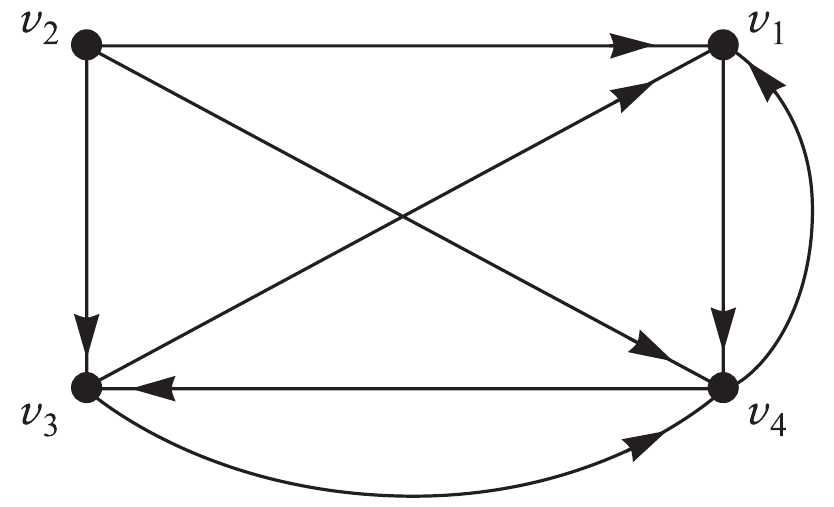
\includegraphics[height=3cm,keepaspectratio=true]{./md/fig0904a.png}
		% fig0904a.png: 0x0 pixel, 300dpi, 0.00x0.00 cm, bb=
		\caption{Construya su matriz de adyacencia del digrado anterior.}
		\label{fig:0904a}
	\end{figure}
	
\end{exmp}




La matriz identidad $I_{m}=\left( I_{i,j} \right)$ de dimensi\'on $m\times m$ se define como
$$I_{i,j}
\begin{cases}
	1 & i=j \\
	0 & i \neq j,
\end{cases}
$$
es decir, es matriz cuadrangular con $1's$ en la \emph{diagonal principal}, y ceros en cualquier otra entrada.



\begin{exmp}
	$$I_{2}=
	\begin{pmatrix}
		1 & 0 \\
		0 & 1 \\
	\end{pmatrix}
	$$
	
	$$I_{3}=
	\begin{pmatrix}
		1 & 0 & 0 \\
		0 & 1 & 0 \\
		0 & 0 & 1
	\end{pmatrix}
	$$
\end{exmp}




La propiedad principal de una matriz identidad $I_{m}$ es que es nuestra respecto a la multiplicaci\'on de matrices, es decir, para cualquier otra matriz $A\in M_{n}:$
$$
AI_{n}=I_{n}A=A.
$$



La potencia $n-$\'esima de una matriz $A \in M_{n}$ se define de manera recursiva como
$$
A^{n}=
\begin{cases}
	I_{n}  & n=0\\
	AA^{n-1} & n \in \N.
\end{cases}
$$ 

Es decir, $$A^{0}=I, A^{1}=A, A^{2}=AA,...$$



Definamos $a_{k}(i,j)$ como la entrada en la posici\'on $i,j$ de $A^{k}.$


\begin{prop}
	Sea $A$ la matriz de adyacencia de un grafo $G.$ Entonces $a_{k}(i,j)$ es igual al n\'umero de caminos de longitud $k$ que van de $v_{i}$ a $v_{j}.$
\end{prop}



{Ejemplo}
Consideremos nuevamente el grafo
\begin{figure}[h]
	\centering
	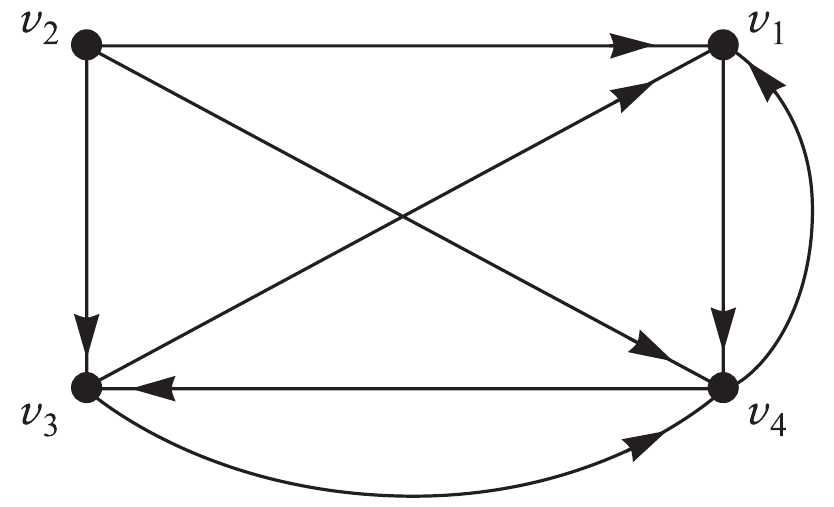
\includegraphics[height=3cm,keepaspectratio=true]{./md/fig0904a.png}
	% fig0904a.png: 0x0 pixel, 300dpi, 0.00x0.00 cm, bb=
\end{figure}



Recordemos que su matriz de adyacencia es
\begin{equation}
	\label{exmp:adj}
	\tag{AD}
	A= \left(\begin{array}{rrrr}
		0 & 0 & 0 & 1 \\
		1 & 0 & 1 & 1 \\
		1 & 0 & 0 & 1 \\
		1 & 0 & 1 & 0
	\end{array}\right)
\end{equation}




Entonces
$$
A^{2}= \left(\begin{array}{rrrr}
	1 & 0 & 1 & 0 \\
	2 & 0 & 1 & 2 \\
	1 & 0 & 1 & 1 \\
	1 & 0 & 0 & 2
\end{array}\right) \;
A^{3}= \left(\begin{array}{rrrr}
	1 & 0 & 0 & 2 \\
	3 & 0 & 2 & 3 \\
	2 & 0 & 1 & 2 \\
	2 & 0 & 2 & 1
\end{array}\right) \;
$$

$$
A^{4}= \left(\begin{array}{rrrr}
	2 & 0 & 2 & 1 \\
	5 & 0 & 3 & 5 \\
	3 & 0 & 2 & 3 \\
	3 & 0 & 1 & 4
\end{array}\right)
$$



Observe que $a_{2}(4,1)=1,$ de manera que existe un solo camino de longitud 2 de $v_{4}$ a $v_{1}.$ De manera similar, como $a_{3}(2,3)=2,$ entonces existen dos caminos de longitud $3$ de $v_{2}$ a $v_{3}.$



\begin{rem}
	Si definimos 
	$$B_{r}= \sum_{i=1}^{r}A^{i},$$
	entonces la entrada $i,j$ de esta matriz nos indicar\'a el n\'umero de caminos de longitud a lo m\'as $r$ de $v_{i}$ a $v_{j}.$
\end{rem}



En nuestro ejemplo, considerando $A$ dado por \eqref{exmp:adj}, tenemos que 
\begin{equation}
	\label{B4}
	B_{4}=
	\left(\begin{array}{rrrr}
		4 & 0 & 3 & 4 \\
		11 & 0 & 7 & 11 \\
		7 & 0 & 4 & 7 \\
		7 & 0 & 4 & 7
	\end{array}\right)
\end{equation}


?`Existe alguna manera de llegar al vertice $v_{2}$ desde el v\'ertice $v_{1}$, sin importar la longitud del camino?


\subsection{Matriz de accesibilidad}


Sea $G=G(V,E)$ un grafo simple dirigido con $m$ v\'ertices $v_{1},...,v_{m}.$ La \emph{matriz de accesibilidad} de $G$ es la matriz $m-$cuadrangular $P=\left( p_{ij} \right)$ definida de la siguiente manera:
$$p_{ij}=
\begin{cases}
	1 & \texttt{existe un camino de }v_{i}\texttt{ a }v_{j}\\
	0 & \texttt{en otro caso}
\end{cases}
$$



\begin{prop}
	Sea $A$ la matriz de adyacencia de un grafo $G$ con $m$ v\'ertices. Entonces la matriz de accesibilidad y 
	\begin{equation}
		\label{Bm}
		B_{m}=\sum_{i=1}^{m}A^{i}
	\end{equation}
	tienen exactamente las mismas entradas no nulas. 
\end{prop}




\begin{defn}
	Un digrafo es \emph{fuertemente conexo} si para cualquier par de v\'ertices $u,v$ existe al menos un camino de $u$ a $v$ y otro de $v$ a $u.$
\end{defn}




\begin{prop}
	Sea $A\in M_{m}$ la matriz de adyacencia de un grafo $G.$ Entonces, las siguientes proposiciones son equivalentes:
	\begin{enumerate}
		\item $G$ es fuertemente conexo;
		\item la matriz de accesibilidad $P$ no tiene entradas nulas;
		\item la matriz $B_{m},$ dada por \eqref{Bm}, no tiene entradas nulas.
	\end{enumerate}
	
\end{prop}




\begin{exmp}
	\label{lip:exmp:0908}
	Para encontrar la matriz de accesibilidad asociada a la matriz de adyacencia $A,$ dada por \eqref{exmp:adj}, basta sustitur las entradas no nulas en la matriz $B_{4},$ dada por \eqref{B4}, por $1's:$
	$$
	P=
	\left(\begin{array}{rrrr}
		1 & 0 & 1 & 1 \\
		1 & 0 & 1 & 1 \\
		1 & 0 & 1 & 1 \\
		1 & 0 & 1 & 1
	\end{array}\right)
	$$
\end{exmp}




\bibliography{_biblio}{}
\bibliographystyle{apa}
\end{document}